% =============================================================================
%   Chapter 4: Maintenance of Zonally Averaged Wind, Temperature,
%              Potential Vorticity, and EP Flux
% =============================================================================

\section{Maintenance of the Zonally Symmetric Circulation}

This chapter addresses the central question of \textit{how} the observed
zonally averaged distributions of temperature, wind, and potential vorticity
are maintained against dissipative processes.  The key players are the
\textbf{eddy fluxes}---the statistical covariances between departures from the
zonal mean---together with diabatic heating and surface friction.

\hisu{이 장의 핵심 질문: 관측된 동서 평균 상태는 어떻게 유지되는가?  에디 플럭스, 복사 가열, 마찰의 균형!}

% =============================================================================
%   SECTION 1 — Maintenance of Zonally Averaged Temperature
% =============================================================================

\subsection{Maintenance of Zonally Averaged Temperature}

% ---- Notation ----
Throughout this chapter we use the following notation conventions.

\begin{definition}[Zonal-Mean and Eddy Decomposition]
For any atmospheric variable $a(\lambda,\phi,p,t)$,
\[
  a = a_Z + a_E,
  \qquad
  a_Z \equiv \frac{1}{2\pi}\int_0^{2\pi} a\,d\lambda,
  \qquad
  (a_E)_Z = 0.
\]
Here $(\cdot)_Z$ denotes the \textgr{zonal average} and $(\cdot)_E$ the
\textgr{eddy (departure)} component.  When a time mean is additionally taken
we write $(\cdot)_{ZM}$.
\end{definition}

\hisu{Zonal mean: 경도 방향으로 한 바퀴 평균.  Eddy: 그 평균으로부터의 편차.  시간 평균까지 하면 ZM.}

\begin{figure}[ht]
  \centering
  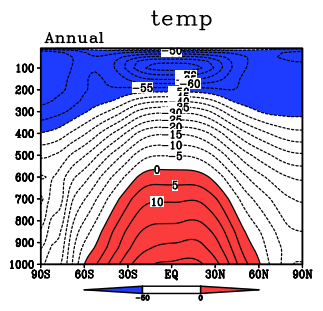
\includegraphics[width=0.85\textwidth]{images/ch04/p05_img01.png}
  \caption{Zonal-mean temperature cross-section (annual mean) as a function of latitude and pressure.  Warm temperatures (red) in the tropical lower troposphere and cold temperatures (blue) in the upper troposphere and polar regions illustrate the equator-to-pole temperature gradient that the general circulation must maintain. \hisu{연평균 동서 평균 온도 단면도.  적도 하층 대류권의 고온과 극지방/상층 대류권의 저온이 일반 순환의 원동력이 되는 적도--극 온도 경도를 보여준다.}}
  \label{fig:ch04_temp_xsec}
\end{figure}

% --------------------------------------------------------------------------
\subsubsection{Thermodynamic Energy Equation}

The first law of thermodynamics applied to an ideal-gas atmosphere in
pressure coordinates gives

\begin{equation}\label{eq:thermo_full}
  \frac{\partial T}{\partial t}
    + \mathbf{V}\cdot\nabla T
    + \omega\frac{\partial T}{\partial p}
    - \frac{1}{c_p}\alpha\omega
  = \frac{1}{c_p}H,
\end{equation}

\noindent
where $\mathbf{V} = (u,v)$ is the horizontal wind, $\omega = Dp/Dt$
is the pressure-coordinate vertical velocity, $\alpha = 1/\rho$ is the
specific volume, and $H$ collects all diabatic heating rates
(radiation, latent heat, sensible heat flux).

\begin{hisublock}
좌변 각 항의 의미:
\begin{itemize}
  \item $\partial T/\partial t$: 국지적 온도 변화율
  \item $\mathbf{V}\cdot\nabla T$: 수평 이류에 의한 온도 변화
  \item $\omega\,\partial T/\partial p$: 연직 이류에 의한 온도 변화
  \item $-(1/c_p)\alpha\omega$: 단열 팽창/압축에 의한 온도 변화 ($\omega<0$이면 상승, 팽창 냉각)
\end{itemize}
\end{hisublock}

\noindent
Using the equation of state $\alpha = RT/p$ we rewrite the adiabatic
compression term:
\[
  \frac{1}{c_p}\alpha\omega = \frac{R\omega T}{c_p p}.
\]

% --------------------------------------------------------------------------
\subsubsection{Flux Form of the Thermodynamic Equation}

The continuity equation in pressure coordinates states
\begin{equation}\label{eq:continuity}
  \nabla\cdot\mathbf{V} + \frac{\partial\omega}{\partial p} = 0.
\end{equation}
Multiplying \eqref{eq:continuity} by $T$ and adding to \eqref{eq:thermo_full}
converts the advection terms to \textgr{flux form}:

\begin{equation}\label{eq:thermo_flux}
  \boxed{
  \frac{\partial T}{\partial t}
    + \nabla\cdot(\mathbf{V}T)
    + \frac{\partial}{\partial p}(\omega T)
    - \frac{R}{c_p\,p}\,\omega T
  = \frac{1}{c_p}H.
  }
\end{equation}

\begin{remark}
The flux form is essential because zonal averaging and vertical
integration commute cleanly with the divergence operators.
\end{remark}

% --------------------------------------------------------------------------
\subsubsection{Zonal Averaging}

\begin{proposition}[Vanishing of Zonal Derivatives]
For any periodic function $a(\lambda)$ with period $2\pi$,
\begin{equation}\label{eq:zonal_deriv_vanish}
  \left(\frac{\partial a}{\partial \lambda}\right)_Z = 0.
\end{equation}
\end{proposition}

\hisu{주기 함수의 한 주기 적분은 항상 0.  이것이 zonal averaging의 핵심 성질!}

\begin{proof}
\[
  \left(\frac{\partial a}{\partial \lambda}\right)_Z
  = \frac{1}{2\pi}\int_0^{2\pi}\frac{\partial a}{\partial\lambda}\,d\lambda
  = \frac{1}{2\pi}\bigl[a(2\pi)-a(0)\bigr] = 0.\qedhere
\]
\end{proof}

\noindent
Expanding the horizontal divergence in spherical coordinates,
\[
  \nabla\cdot(\mathbf{V}T)
  = \frac{1}{a\cos\phi}\frac{\partial(uT)}{\partial\lambda}
    + \frac{1}{a\cos\phi}\frac{\partial}{\partial\phi}(vT\cos\phi),
\]
the first term vanishes upon zonal averaging by \eqref{eq:zonal_deriv_vanish}.
Thus the \textgr{zonally averaged thermodynamic equation} is

\begin{equation}\label{eq:thermo_zonal}
  \frac{\partial T_Z}{\partial t}
    + \frac{1}{a\cos\phi}\frac{\partial}{\partial\phi}\bigl((vT)_Z\cos\phi\bigr)
    + \frac{\partial}{\partial p}(\omega T)_Z
    - \frac{R}{c_p\,p}(\omega T)_Z
  = \frac{1}{c_p}H_Z.
\end{equation}

% --------------------------------------------------------------------------
\subsubsection{Vertical Averaging and Boundary Conditions}

Integrating \eqref{eq:thermo_zonal} from $p=0$ (top of atmosphere) to
$p=p_0$ (surface) and applying the boundary conditions
\begin{equation}\label{eq:omega_bc}
  \omega = 0 \quad\text{at } p=0 \quad\text{and}\quad p=p_0,
\end{equation}
the vertical flux divergence integrates out:
\[
  \int_0^{p_0}\frac{\partial}{\partial p}(\omega T)_Z\,dp
  = \bigl[(\omega T)_Z\bigr]_0^{p_0} = 0.
\]

\begin{hisublock}
$\omega=0$인 경계 조건:
\begin{itemize}
  \item $p=0$ (대기 상한): 대기 위에 물질이 없으므로 $\omega=0$
  \item $p=p_0$ (지표): 지표면이 평평하고 움직이지 않으므로 $\omega\approx 0$
\end{itemize}
이 경계 조건을 적용하면 $\omega T$의 연직 플럭스 발산 항이 적분 시 사라진다.
\end{hisublock}

\noindent
Similarly, define the vertical mean
$\langle\cdot\rangle \equiv \frac{1}{p_0}\int_0^{p_0}(\cdot)\,dp$.
The adiabatic compression term integrates to
\[
  \frac{R}{c_p\,p_0}\int_0^{p_0}\frac{(\omega T)_Z}{p}\,dp \approx 0,
\]
because the boundary conditions force $\omega T$ to vanish at both limits and
the integrand is small in between (to leading order).  Therefore the
\textgr{vertically and zonally averaged} thermodynamic equation becomes

\begin{equation}\label{eq:thermo_ZV}
  \boxed{
  \frac{\partial\langle T_Z\rangle}{\partial t}
    + \frac{1}{a\cos\phi}\frac{\partial}{\partial\phi}
      \bigl(\langle(vT)_Z\rangle\cos\phi\bigr)
  = \frac{1}{c_p}\langle H_Z\rangle.
  }
\end{equation}

% --------------------------------------------------------------------------
\subsubsection{Decomposition of the Meridional Heat Flux}

Using $v = v_Z + v_E$ and $T = T_Z + T_E$:
\begin{equation}\label{eq:heat_flux_decomp}
  (vT)_Z = v_Z\,T_Z + (v_E\,T_E)_Z.
\end{equation}

\begin{remark}[Mean-Flow Contribution is Negligible]
For quasi-geostrophic flow, the geostrophic meridional wind $v_g$ satisfies
\[
  v_g = \frac{1}{f}\frac{1}{a}\frac{\partial\Phi}{\partial\lambda},
\]
and upon zonal averaging,
\[
  (v_g)_Z = \frac{1}{f}\frac{1}{a}
    \left(\frac{\partial\Phi}{\partial\lambda}\right)_Z = 0
  \quad\text{by \eqref{eq:zonal_deriv_vanish}}.
\]
Hence $v_Z \approx 0$, and the mean-flow heat flux
$v_Z\,T_Z \approx 0$.
\end{remark}

\hisu{지균 균형이면 $v$의 동서 평균은 거의 0.  따라서 열 수송은 거의 전부 에디에 의한 것!}

\noindent
Therefore
\begin{equation}\label{eq:heat_flux_eddy}
  (vT)_Z \approx (v_E\,T_E)_Z.
\end{equation}

\begin{figure}[ht]
  \centering
  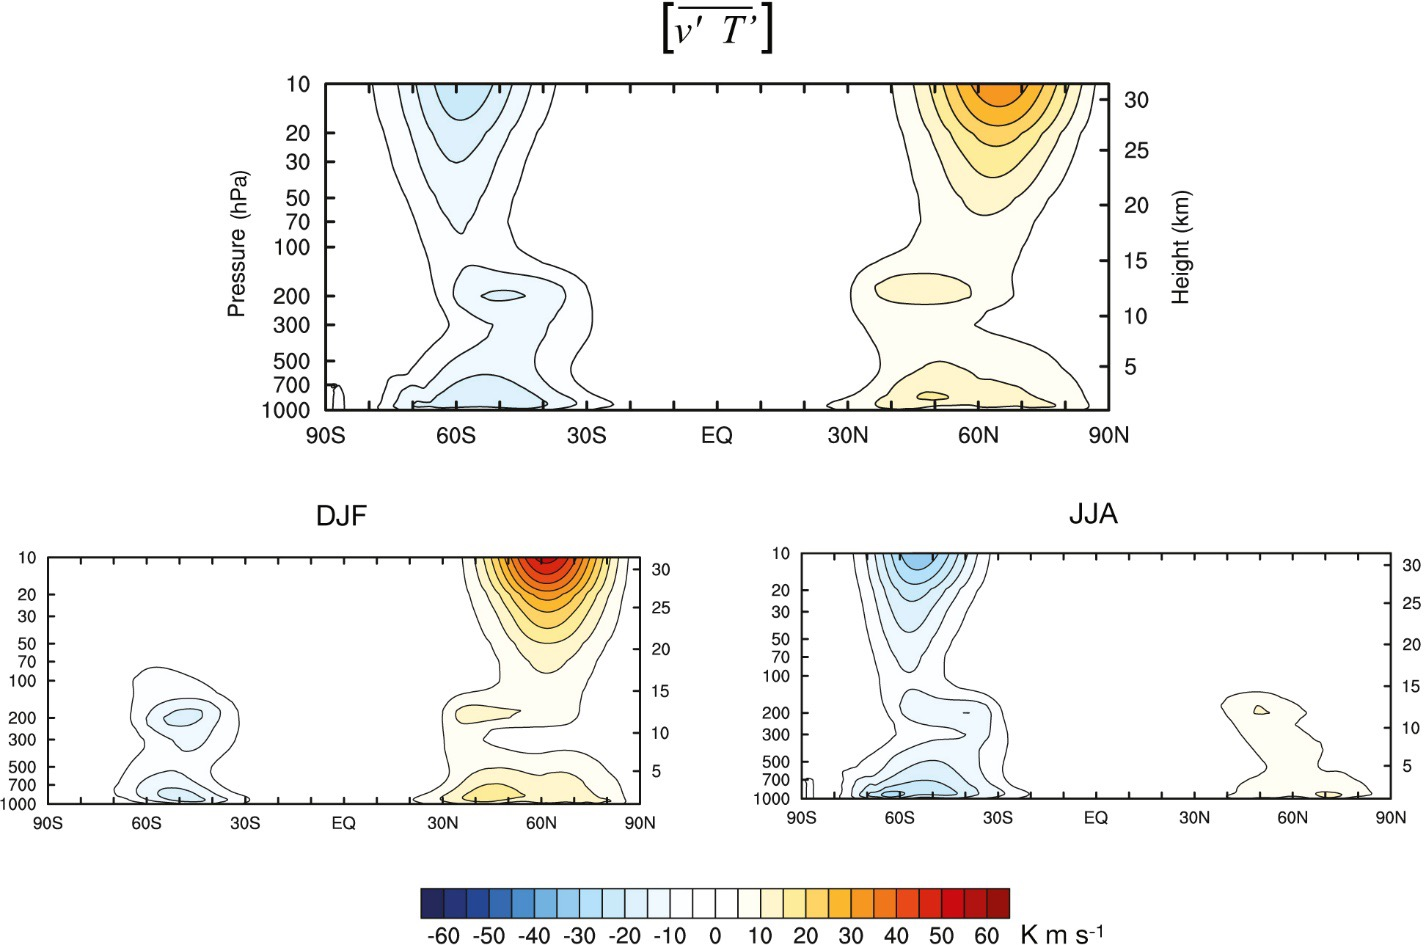
\includegraphics[width=0.85\textwidth]{images/ch04/p76_img01.jpeg}
  \caption{Observed zonal-mean transient eddy heat flux $\overline{[v'T']}$ (K\,m\,s$^{-1}$) cross-section: annual mean (top), DJF (bottom left), and JJA (bottom right).  Poleward heat flux maxima appear in the midlatitude lower troposphere ($\sim$40--60$^\circ$, 700--850\,hPa), strongest in the winter hemisphere, confirming that transient eddies dominate the meridional heat transport. \hisu{이동성 에디 열 플럭스 $[v'T']$ 관측 단면도.  중위도 하층 대류권에서 극 방향 열 수송이 최대이며, 겨울 반구에서 가장 강하다.  에디가 열 수송을 지배한다는 이론적 결과와 일치.}}
  \label{fig:ch04_transient_heat_flux}
\end{figure}

% --------------------------------------------------------------------------
\subsubsection{Steady-State Balance}

Taking a \textbf{time mean} of \eqref{eq:thermo_ZV} and assuming a
\textgr{statistically steady state} ($\partial\langle T_Z\rangle/\partial t = 0$):

\begin{equation}\label{eq:thermo_steady}
  \boxed{
  \frac{1}{a\cos\phi}\frac{\partial}{\partial\phi}
    \Bigl(\overline{(vT)}_{ZM}\cos\phi\Bigr)
  \approx \frac{1}{c_p}\overline{H}_{ZM}.
  }
\end{equation}

\begin{theorem}[Steady-State Heat Balance]
In the time-mean, zonally and vertically averaged thermodynamic balance,
the convergence of the meridional heat transport balances diabatic
heating.  Since the mean-flow contribution to $\overline{(vT)}_{ZM}$ is
negligible, the balance is between \textgr{eddy heat transport} and
diabatic heating:
\[
  \frac{1}{a\cos\phi}\frac{\partial}{\partial\phi}
    \Bigl(\overline{(v_E T_E)}_{ZM}\cos\phi\Bigr)
  \approx \frac{1}{c_p}\overline{H}_{ZM}.
\]
\end{theorem}

\hisu{열 수송 $\approx$ 에디에 의한 수송이 지배적.  평균 흐름의 기여는 무시할 수 있다.
정상 상태에서 에디 열 수송의 수렴 = 당뇨 가열 (복사 냉각/가열).}

\begin{figure}[ht]
  \centering
  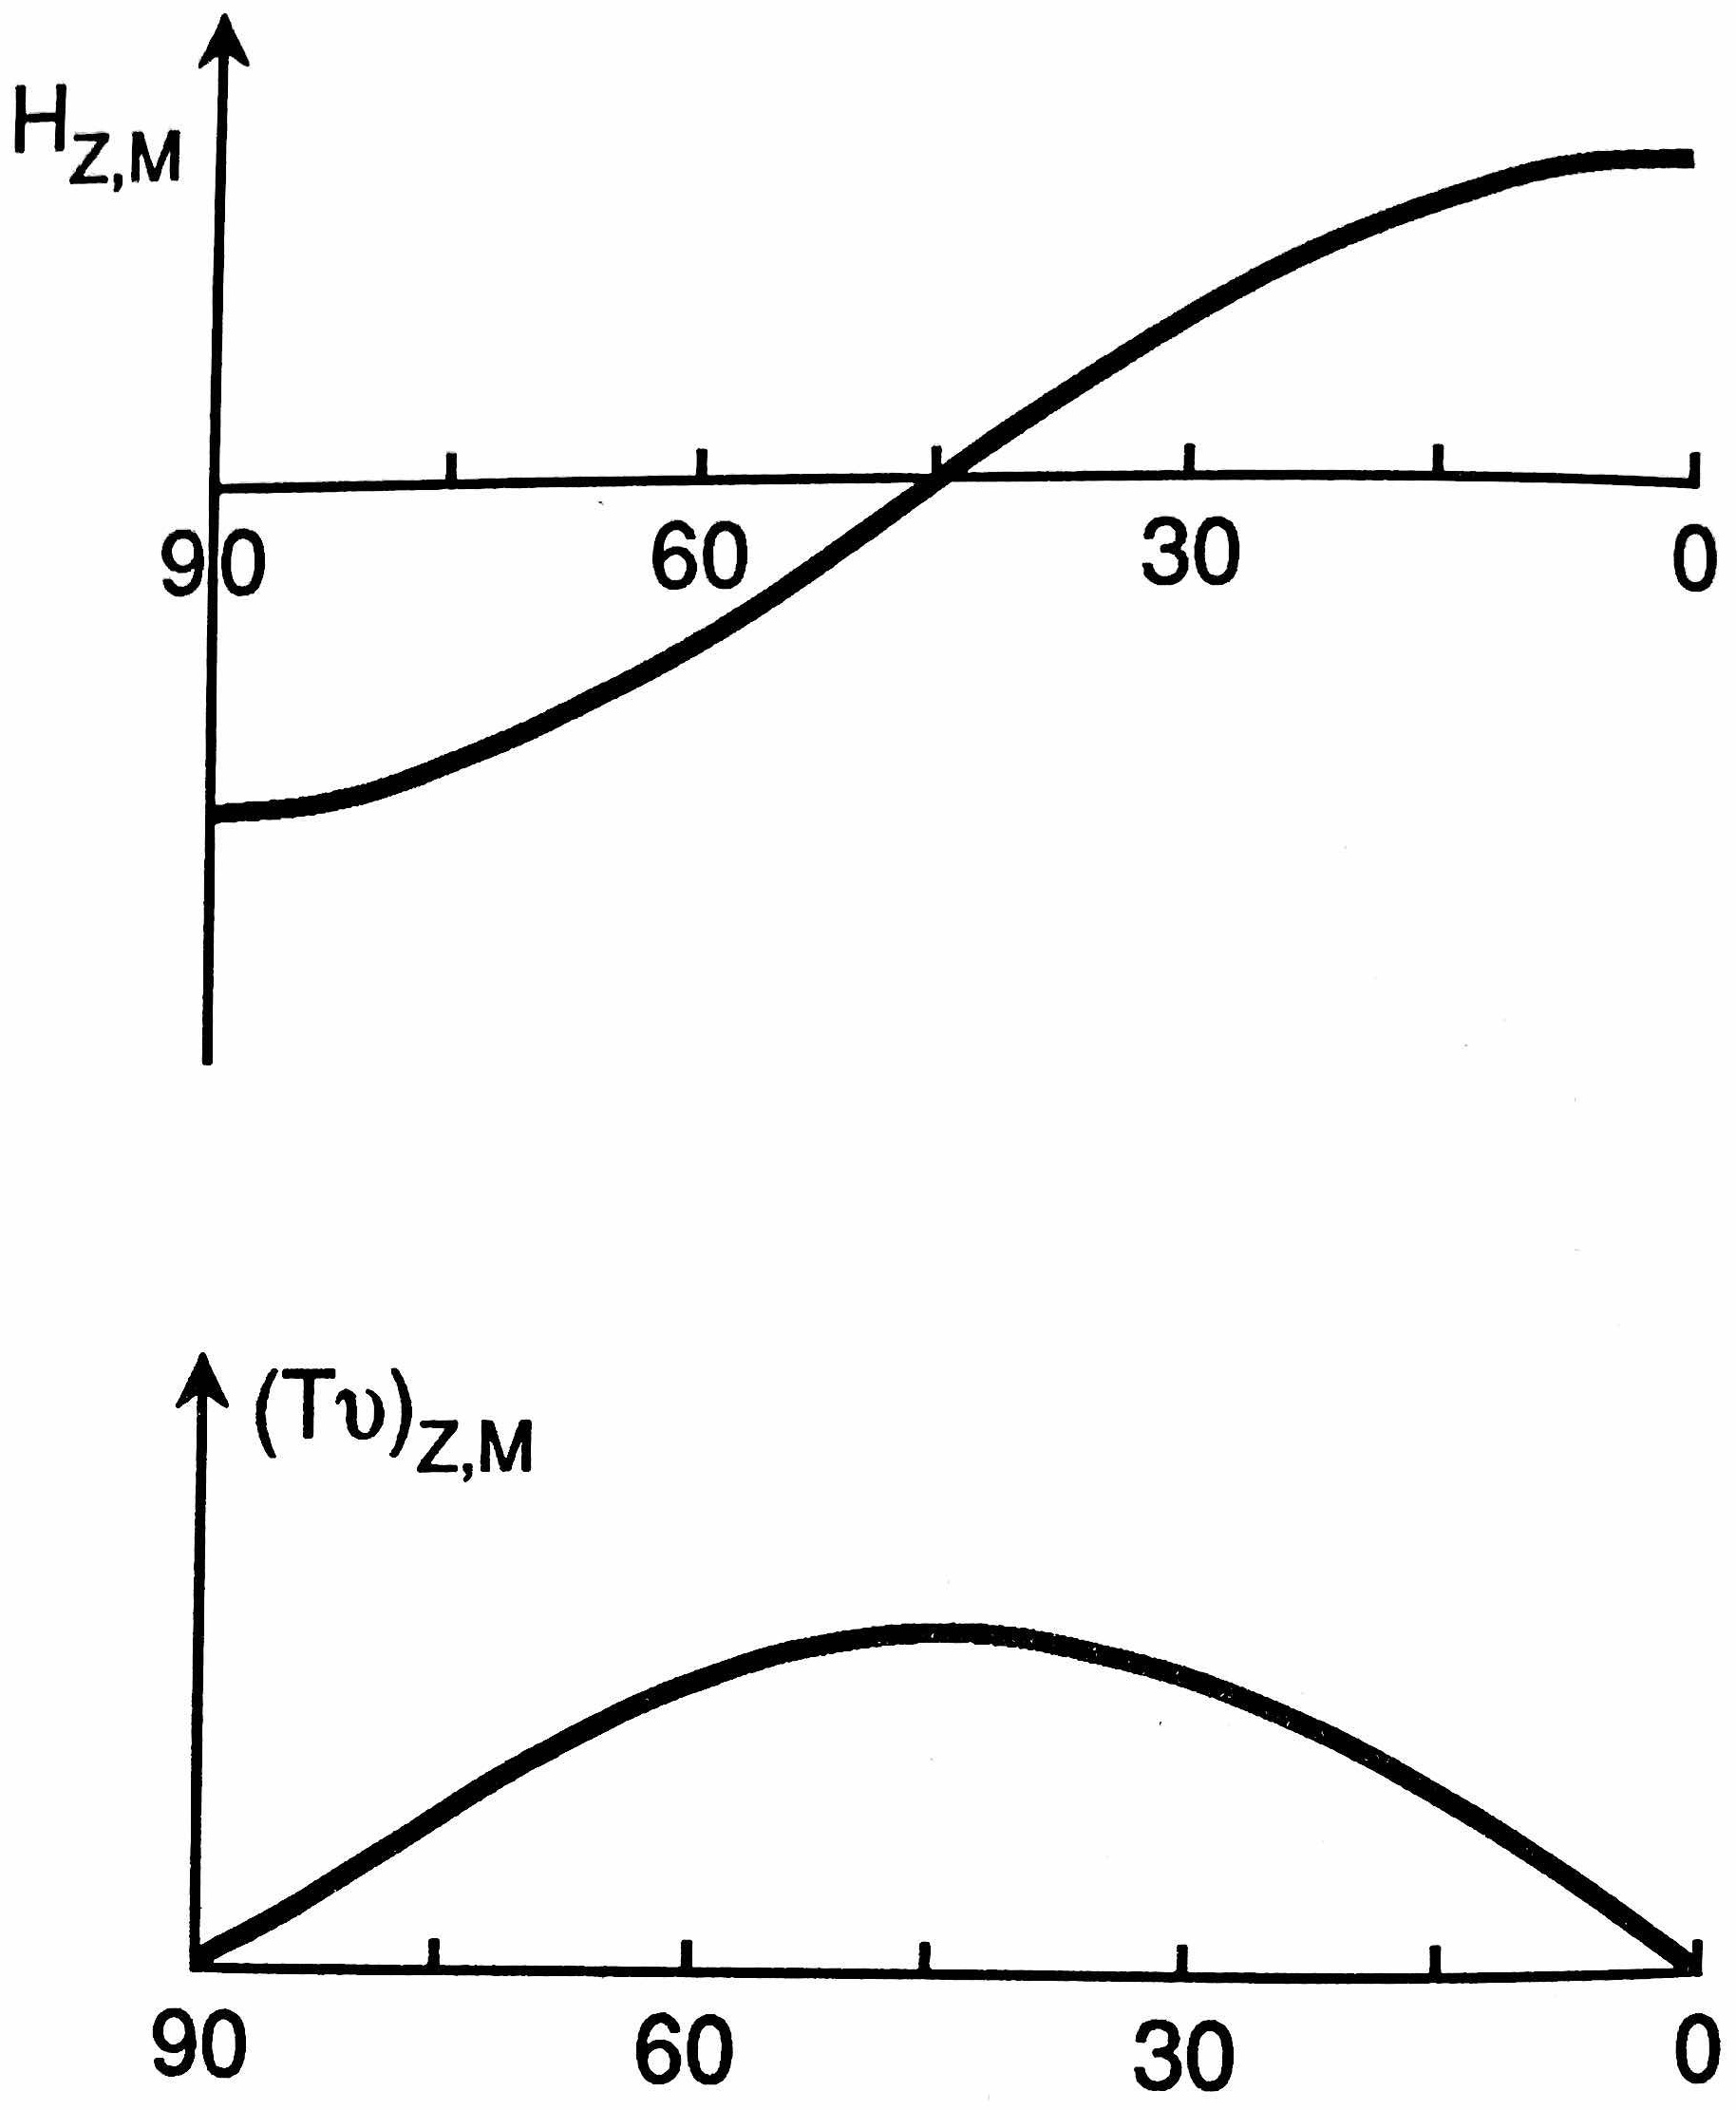
\includegraphics[width=0.75\textwidth]{images/ch04/p14_img01.jpeg}
  \caption{Idealized profiles of the zonally and vertically averaged diabatic heating $H_{ZM}$ (top) and meridional heat transport $(Tv)_{ZM}$ (bottom) as functions of latitude.  Diabatic heating is positive (warming) in the tropics and negative (radiative cooling) at high latitudes; the implied poleward heat transport peaks in the midlatitudes near $\sim$40$^\circ$. \hisu{이상적인 당뇨 가열 $H_{ZM}$ (위)과 자오면 열 수송 $(Tv)_{ZM}$ (아래)의 위도별 분포.  열대에서 가열, 고위도에서 냉각이며, 이를 균형시키는 극 방향 열 수송은 중위도에서 최대.}}
  \label{fig:ch04_diabatic_heating}
\end{figure}


% =============================================================================
%   SECTION 2 — Maintenance of Zonally Averaged Wind
% =============================================================================

\subsection{Maintenance of Zonally Averaged Wind}

\begin{figure}[ht]
  \centering
  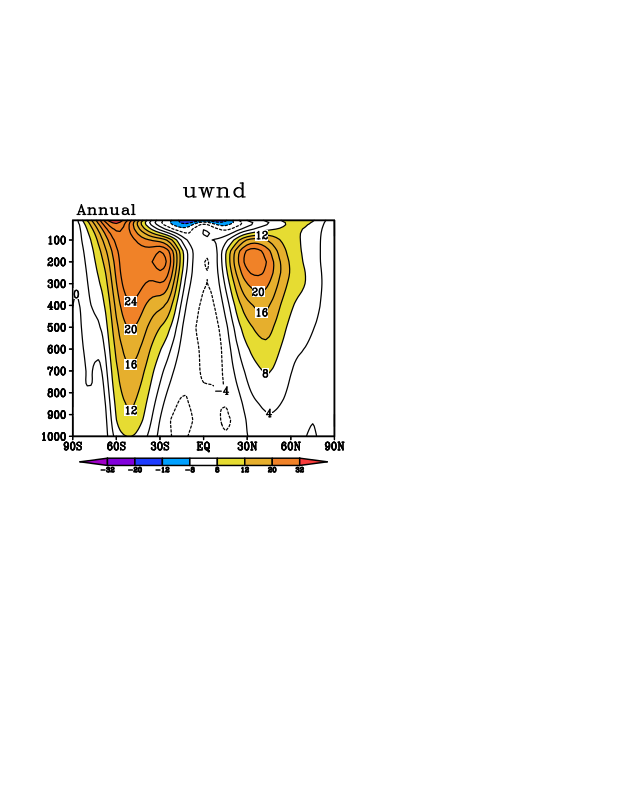
\includegraphics[width=0.85\textwidth]{images/ch04/p16_img01.png}
  \caption{Zonal-mean zonal wind cross-section (annual mean, m\,s$^{-1}$) as a function of latitude and pressure.  The subtropical jet streams appear as westerly maxima ($>$24\,m\,s$^{-1}$) near 200\,hPa at $\sim$30$^\circ$ in both hemispheres, with easterlies in the tropical upper troposphere and weak surface westerlies in the midlatitudes. \hisu{연평균 동서 평균 동서풍 단면도.  아열대 제트류가 양 반구 $\sim$30$^\circ$, 200\,hPa 부근에서 서풍 극대로 나타나며, 열대 상층에는 동풍이, 중위도 지표에는 약한 서풍이 존재한다.}}
  \label{fig:ch04_uwind_xsec}
\end{figure}

% --------------------------------------------------------------------------
\subsubsection{Zonal Momentum Equation}

The zonal momentum equation in spherical pressure coordinates is

\begin{equation}\label{eq:u_momentum}
  \frac{\partial u}{\partial t}
    + \frac{u}{a\cos\phi}\frac{\partial u}{\partial\lambda}
    + \frac{v}{a}\frac{\partial u}{\partial\phi}
    + \omega\frac{\partial u}{\partial p}
    - \frac{uv\tan\phi}{a}
  = -\frac{1}{a\cos\phi}\frac{\partial\Phi}{\partial\lambda}
    + fv + F_\lambda,
\end{equation}

\noindent
where the $uv\tan\phi/a$ term is the metric (curvature) term arising from
spherical geometry, and $F_\lambda$ represents frictional and other
sub-grid-scale forces.

\begin{hisublock}
좌변 각 항:
\begin{itemize}
  \item $\partial u/\partial t$: 동서 바람의 국지적 변화율
  \item 이류 항 3개: 수평 + 연직 이류
  \item $-uv\tan\phi/a$: 구면 좌표계의 기하학적(metric) 항
\end{itemize}
우변:
\begin{itemize}
  \item $-(a\cos\phi)^{-1}\partial\Phi/\partial\lambda$: 기압경도력
  \item $fv$: 코리올리 힘
  \item $F_\lambda$: 마찰력
\end{itemize}
\end{hisublock}

% --------------------------------------------------------------------------
\subsubsection{Flux Form}

Using the continuity equation \eqref{eq:continuity} and the identity
\[
  v\frac{\partial u}{\partial\phi} - \frac{uv\tan\phi}{a}
  = \frac{1}{a\cos^2\phi}\frac{\partial}{\partial\phi}(uv\cos^2\phi)
    - \frac{u}{a\cos\phi}\frac{\partial}{\partial\phi}(v\cos\phi),
\]
the momentum equation is rewritten in \textgr{flux form}:

\begin{equation}\label{eq:u_flux}
  \boxed{
  \frac{\partial u}{\partial t}
    + \frac{1}{a\cos^2\phi}\frac{\partial}{\partial\phi}(uv\cos^2\phi)
    + \frac{\partial}{\partial p}(u\omega)
  = -\frac{1}{a\cos\phi}\frac{\partial\Phi}{\partial\lambda}
    + fv + F_\lambda.
  }
\end{equation}

% --------------------------------------------------------------------------
\subsubsection{Zonally and Vertically Averaged Equation}

Applying zonal averaging to \eqref{eq:u_flux}:
\begin{itemize}
  \item The pressure-gradient term vanishes:
    $\displaystyle\left(\frac{1}{a\cos\phi}\frac{\partial\Phi}{\partial\lambda}\right)_Z = 0$
    by \eqref{eq:zonal_deriv_vanish}.
  \item The Coriolis term: $f v_Z \approx 0$ (geostrophic balance $\Rightarrow v_Z \approx 0$).
\end{itemize}

\noindent
Integrating vertically with boundary conditions \eqref{eq:omega_bc}:

\begin{equation}\label{eq:u_ZV}
  \boxed{
  \frac{\partial\langle u_Z\rangle}{\partial t}
  = -\frac{1}{a\cos^2\phi}\frac{\partial}{\partial\phi}
    \bigl(\langle(uv)_Z\rangle\cos^2\phi\bigr)
    + \langle F_{\lambda Z}\rangle.
  }
\end{equation}

\hisu{동서 평균 바람의 시간 변화 = 운동량 플럭스의 수렴 + 마찰력.
기압경도력과 코리올리 힘은 zonal averaging 후 사라진다!}

% --------------------------------------------------------------------------
\subsubsection{Decomposition of Momentum Flux}

Analogously to the heat flux decomposition,
\begin{equation}\label{eq:mom_flux_decomp}
  (uv)_Z = u_Z\,v_Z + (u_E\,v_E)_Z \approx (u_E\,v_E)_Z,
\end{equation}
since $v_Z \approx 0$ by the geostrophic argument.  The momentum budget is
therefore controlled by \textgr{eddy momentum fluxes}.

\begin{figure}[ht]
  \centering
  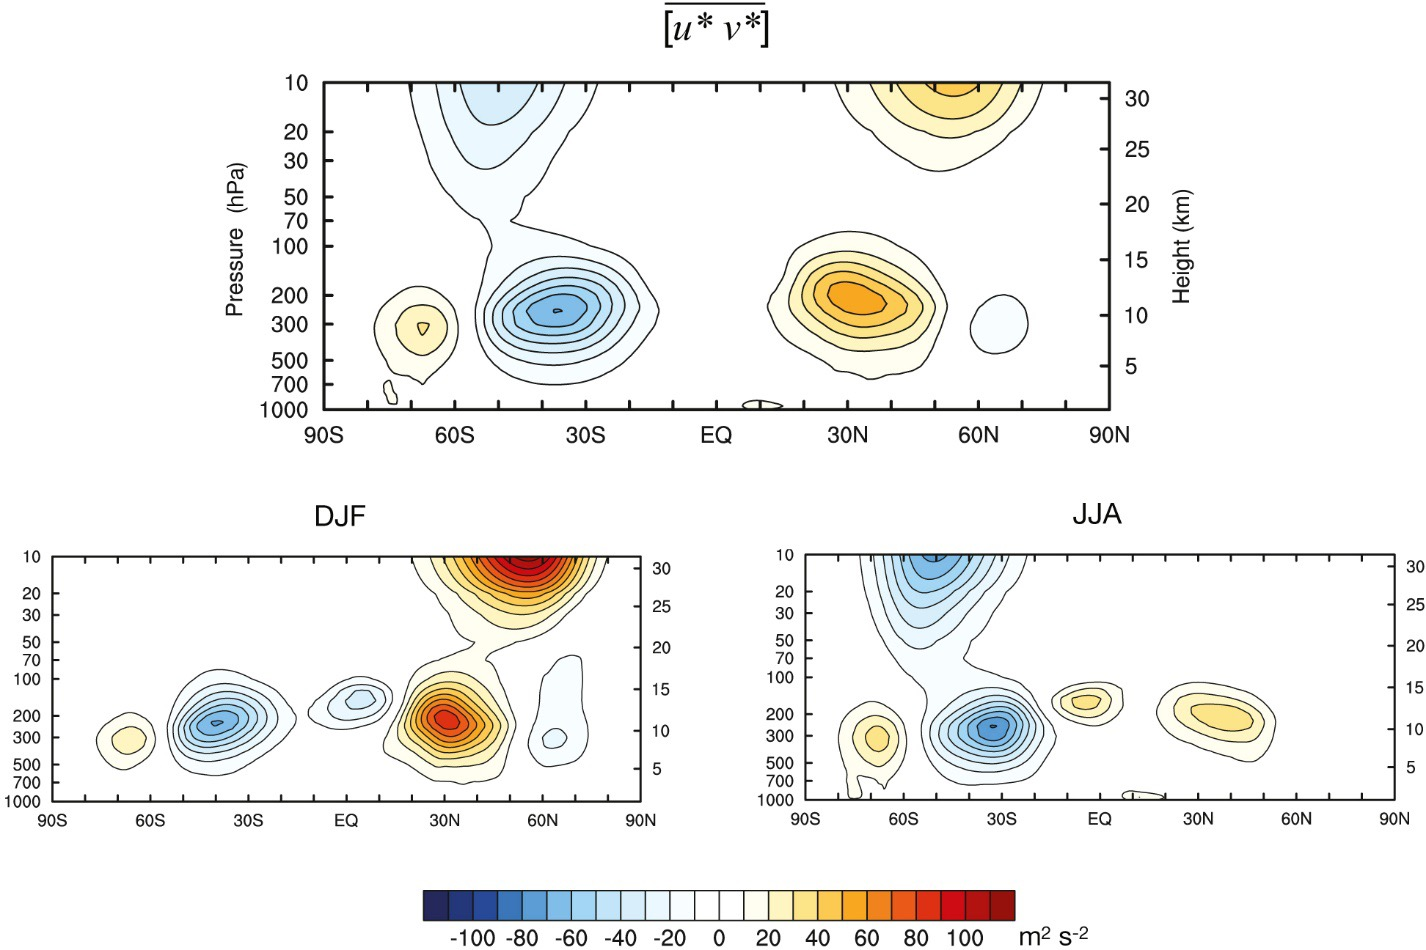
\includegraphics[width=0.85\textwidth]{images/ch04/p71_img01.jpeg}
  \caption{Observed zonal-mean eddy momentum flux $\overline{[u^*v^*]}$ (m$^2$\,s$^{-2}$) cross-section (total eddies = stationary + transient): annual mean (top), DJF (bottom left), and JJA (bottom right).  Positive values indicate poleward momentum transport, which converges into the midlatitude jet region, illustrating the upgradient nature of eddy momentum transport. \hisu{관측된 에디 운동량 플럭스 $[u^*v^*]$ 단면도 (정상파 + 이동성 에디 합).  양의 값은 극 방향 운동량 수송을 나타내며, 중위도 제트류 영역으로 수렴하여 운동량의 upgradient 수송을 보여준다.}}
  \label{fig:ch04_eddy_momentum_flux}
\end{figure}

% --------------------------------------------------------------------------
\subsubsection{Parameterization of Surface Friction}

Friction enters through the stress divergence:

\begin{equation}\label{eq:friction}
  F_\lambda = g\frac{\partial\tau_\lambda}{\partial p},
\end{equation}

\noindent
where $\tau_\lambda$ is the zonal component of the stress tensor.
At the surface, the stress is parameterized by a \textgr{bulk aerodynamic formula}:

\begin{equation}\label{eq:surface_stress}
  \tau_{\lambda Z}(p_0) \approx -C_d\,\rho\,V_0\,u_Z(p_0),
\end{equation}

\noindent
where $C_d$ is the drag coefficient ($\sim 10^{-3}$), and $V_0$ is the
near-surface wind speed.  Integrating \eqref{eq:friction} vertically and
linearizing:

\begin{equation}\label{eq:Rayleigh}
  \langle F_{\lambda Z}\rangle \approx -\varepsilon\,u_Z(p_0),
  \qquad
  \varepsilon \approx 3\times 10^{-6}\;\text{s}^{-1}.
\end{equation}

\hisu{$\varepsilon$는 Rayleigh 마찰 계수.  지표 마찰을 선형 감쇠로 근사한 것.
$1/\varepsilon \approx 3.9$일, 즉 약 4일의 감쇠 시간 규모.}

% --------------------------------------------------------------------------
\subsubsection{Steady-State Momentum Balance}

In a time-mean steady state ($\partial\langle u_Z\rangle/\partial t = 0$):

\begin{equation}\label{eq:u_steady}
  \boxed{
  \frac{1}{a\cos^2\phi}\frac{\partial}{\partial\phi}
    \bigl(\overline{(u_Ev_E)}_{ZM}\cos^2\phi\bigr)
  \approx \varepsilon\,\overline{u}_Z(p_0).
  }
\end{equation}

\begin{theorem}[Steady-State Momentum Balance]
The convergence of the eddy momentum flux balances surface friction.
Where momentum flux converges (midlatitudes), westerlies are maintained;
where it diverges (tropics and high latitudes), easterlies or weak
westerlies result.
\end{theorem}

\hisu{운동량 플럭스의 수렴 $\approx$ 소산 (마찰에 의한 소멸).
에디가 운동량을 중위도로 모아서 제트를 유지하고, 마찰이 이를 소산시킨다.}

\begin{figure}[ht]
  \centering
  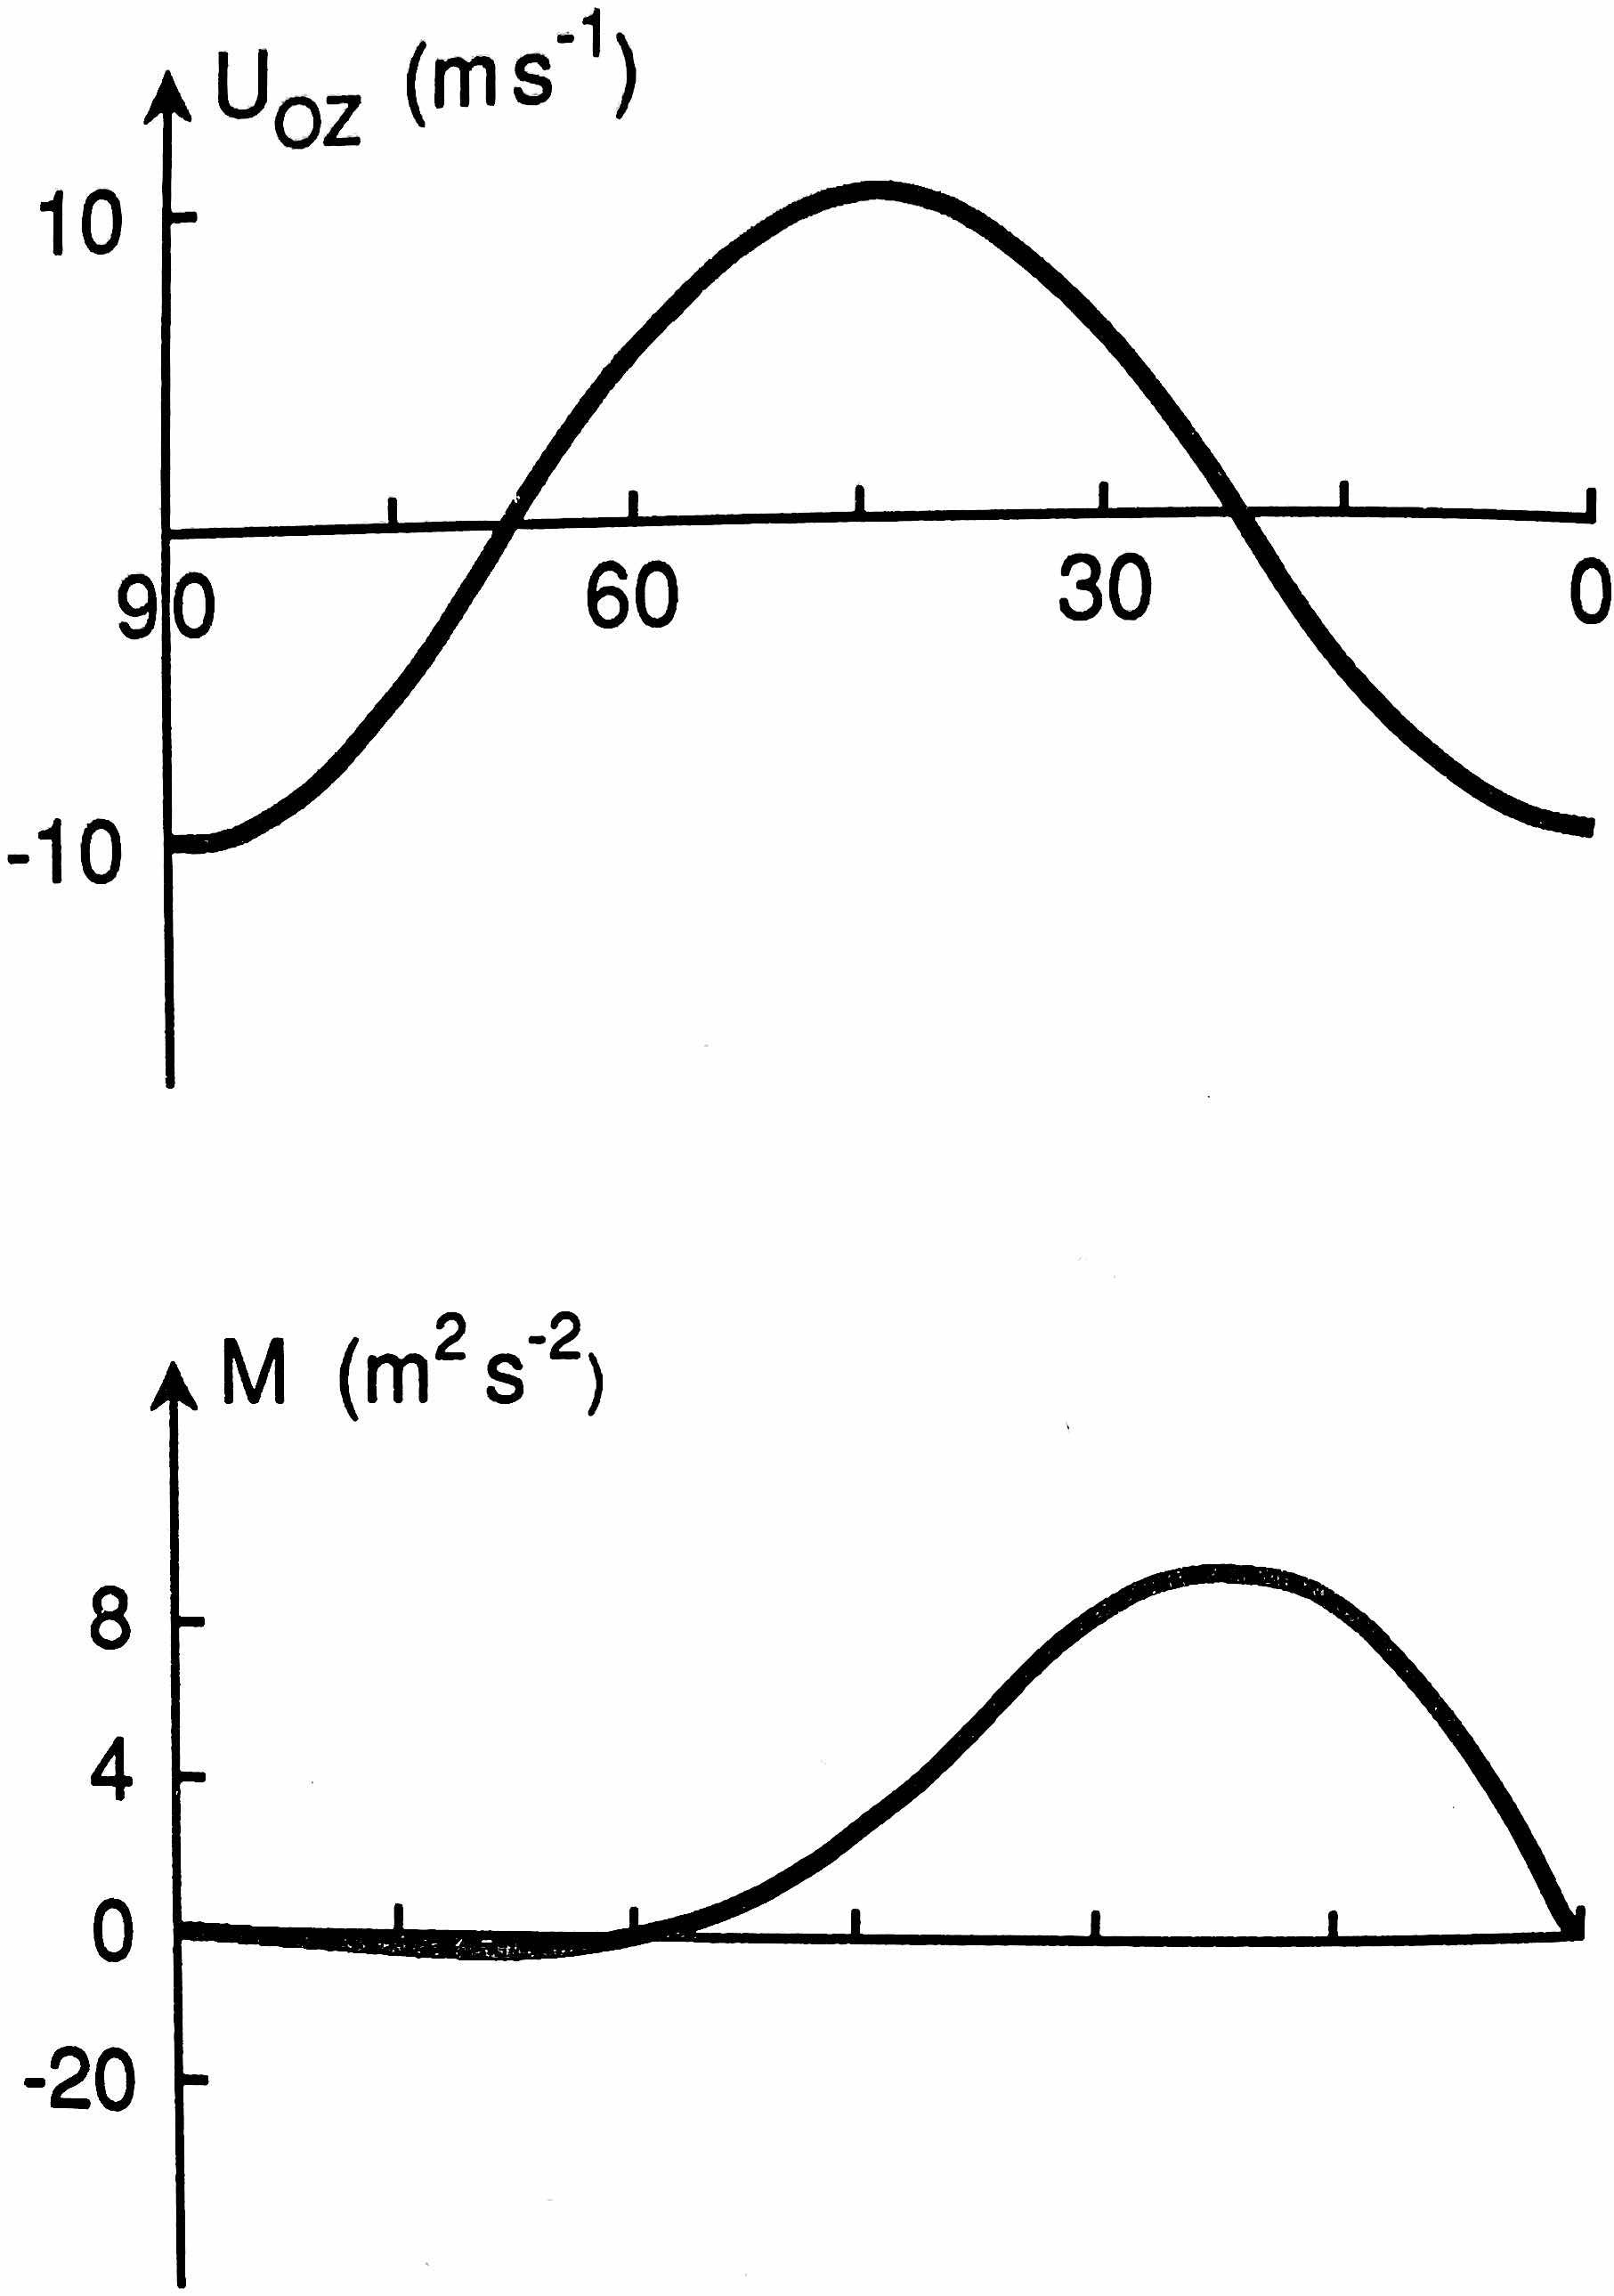
\includegraphics[width=0.75\textwidth]{images/ch04/p27_img01.jpeg}
  \caption{Idealized profiles of the zonal-mean surface zonal wind $U_{OZ}$ (top, m\,s$^{-1}$) and vertically averaged eddy momentum flux $M = \overline{(u_Ev_E)}_{ZM}$ (bottom, m$^2$\,s$^{-2}$) as functions of latitude.  Surface westerlies peak near 45$^\circ$ where momentum flux converges; surface easterlies occur in the tropics and high latitudes where momentum flux diverges. \hisu{이상적인 지표 동서풍 $U_{OZ}$ (위)과 에디 운동량 플럭스 $M$ (아래)의 위도별 분포.  운동량 플럭스가 수렴하는 $\sim$45$^\circ$ 부근에서 지표 서풍이 극대, 발산하는 열대와 고위도에서 동풍.}}
  \label{fig:ch04_surface_wind_momentum}
\end{figure}

% --------------------------------------------------------------------------
\subsubsection{Heat Transport vs.\ Momentum Transport: A Fundamental Contrast}

\begin{multicols}{2}
\textgr{Heat Transport}
\begin{itemize}
  \item \textbf{Downgradient}: warm $\to$ cold (equator $\to$ pole)
  \item $\overline{(v_E T_E)}_{ZM} > 0$ in NH (northward)
  \item Can be parameterized as diffusion:
    $(v_E T_E)_Z \approx -K_T\,\dfrac{1}{a}\dfrac{\partial T_Z}{\partial\phi}$
\end{itemize}

\columnbreak

\textgr{Momentum Transport}
\begin{itemize}
  \item \textbf{Upgradient}: low-$u$ $\to$ high-$u$ regions
  \item From tropics \& high latitudes $\to$ midlatitudes
  \item \textbf{Cannot} be parameterized as simple diffusion
\end{itemize}
\end{multicols}

\hisu{열은 따뜻한 곳에서 차가운 곳으로 (downgradient), 운동량은 반대로 upgradient!
이게 핵심 차이.  열은 확산으로 모사 가능하지만, 운동량은 불가능.
이 차이를 해결하는 열쇠가 바로 PV 수송과 EP 플럭스 이론이다.}

\begin{figure}[ht]
  \centering
  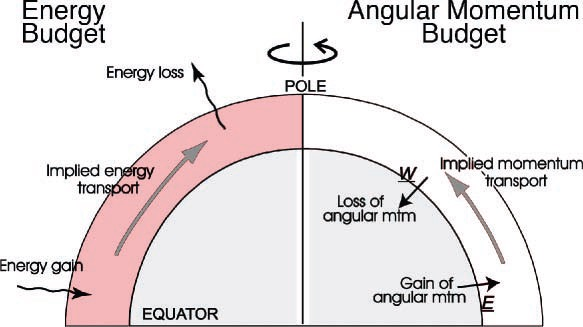
\includegraphics[width=0.85\textwidth]{images/ch04/p29_img01.jpeg}
  \caption{Schematic comparison of the energy budget (left) and the angular momentum budget (right).  In the energy budget, there is a net radiative gain in the tropics and a net loss at the poles, requiring poleward energy transport.  In the angular momentum budget, westerly surface winds at midlatitudes lose angular momentum to friction, while tropical easterlies gain it; eddy momentum transport from the tropics to midlatitudes maintains the balance. \hisu{에너지 수지 (좌)와 각운동량 수지 (우)의 비교 모식도.  에너지는 적도에서 극으로 수송 (복사 불균형 보상), 운동량은 열대와 고위도에서 중위도로 수송 (제트 유지와 마찰 보상).}}
  \label{fig:ch04_energy_vs_momentum}
\end{figure}

\begin{figure}[ht]
  \centering
  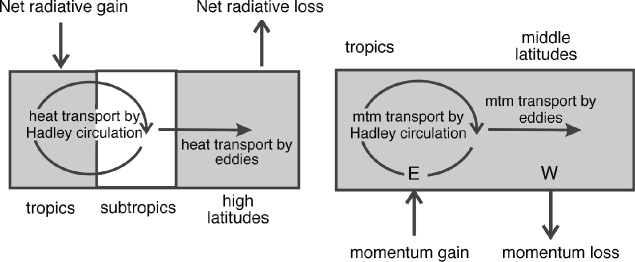
\includegraphics[width=0.85\textwidth]{images/ch04/p31_img01.png}
  \caption{Box-diagram schematic of heat transport (left) and momentum transport (right) in the atmosphere.  Heat is transported poleward by the Hadley circulation in the tropics and by eddies in the extratropics, balancing net radiative gain and loss.  Momentum is transported poleward by the Hadley cell and equatorward by eddies, maintaining tropical easterlies (E) and midlatitude westerlies (W) against surface friction. \hisu{열 수송 (좌)과 운동량 수송 (우)의 박스 모식도.  해들리 순환은 열대에서, 에디는 중고위도에서 열 수송을 담당.  운동량은 해들리 셀이 극 방향으로, 에디가 적도에서 중위도로 수송하여 표면 바람 분포를 유지한다.}}
  \label{fig:ch04_transport_box_schematic}
\end{figure}

% --------------------------------------------------------------------------
\subsubsection{Phase Relationships for Nonzero Fluxes}

For the eddy fluxes to be nonzero in the zonal mean, \textit{systematic
phase relationships} must exist between the wave perturbations.

\begin{proposition}[Phase Condition for Nonzero Heat Flux]
Consider wave-form perturbations
$v_E = \hat{v}\cos(k\lambda - \nu t)$ and
$T_E = \hat{T}\cos(k\lambda - \nu t + \delta)$.
Then
\[
  (v_E\,T_E)_Z = \tfrac{1}{2}\hat{v}\hat{T}\cos\delta.
\]
For nonzero poleward heat flux, $\delta \neq \pm\pi/2$:
\textit{the temperature perturbation must lag the geopotential/velocity
perturbation}.
\end{proposition}

\hisu{$\delta = 0$이면 최대, $\delta = \pm\pi/2$이면 0.
관측에서는 온도가 기압골 뒤에 위치 ($\delta > 0$) $\Rightarrow$ 북쪽으로 열 수송.}

\begin{proposition}[Phase Condition for Nonzero Momentum Flux]
For nonzero $(u_E\,v_E)_Z$, the trough/ridge lines of the wave must be
\textbf{tilted} in the horizontal plane.  In the Northern Hemisphere,
\textgr{NE--SW tilted} trough lines yield northward (poleward)
momentum transport:
\[
  (u_E\,v_E)_Z > 0 \quad\Longleftrightarrow\quad
  \text{NE--SW tilt of trough axes.}
\]
\end{proposition}

\begin{hisublock}
직관적 이해:
\begin{itemize}
  \item 기압골 축이 NE--SW로 기울어져 있으면, 골 서쪽에서는 남서풍 ($u>0, v<0$이 아닌
        $u>0, v>0$ 조합이 우세), 골 동쪽에서는 북서풍이지만 $u<0$.
  \item 결과적으로 $uv > 0$인 영역이 $uv < 0$인 영역보다 넓어서 zonal mean이 양수.
  \item 이 기울기가 없으면 (남북 대칭이면) $(u_Ev_E)_Z = 0$.
\end{itemize}
\end{hisublock}

\begin{figure}[ht]
  \centering
  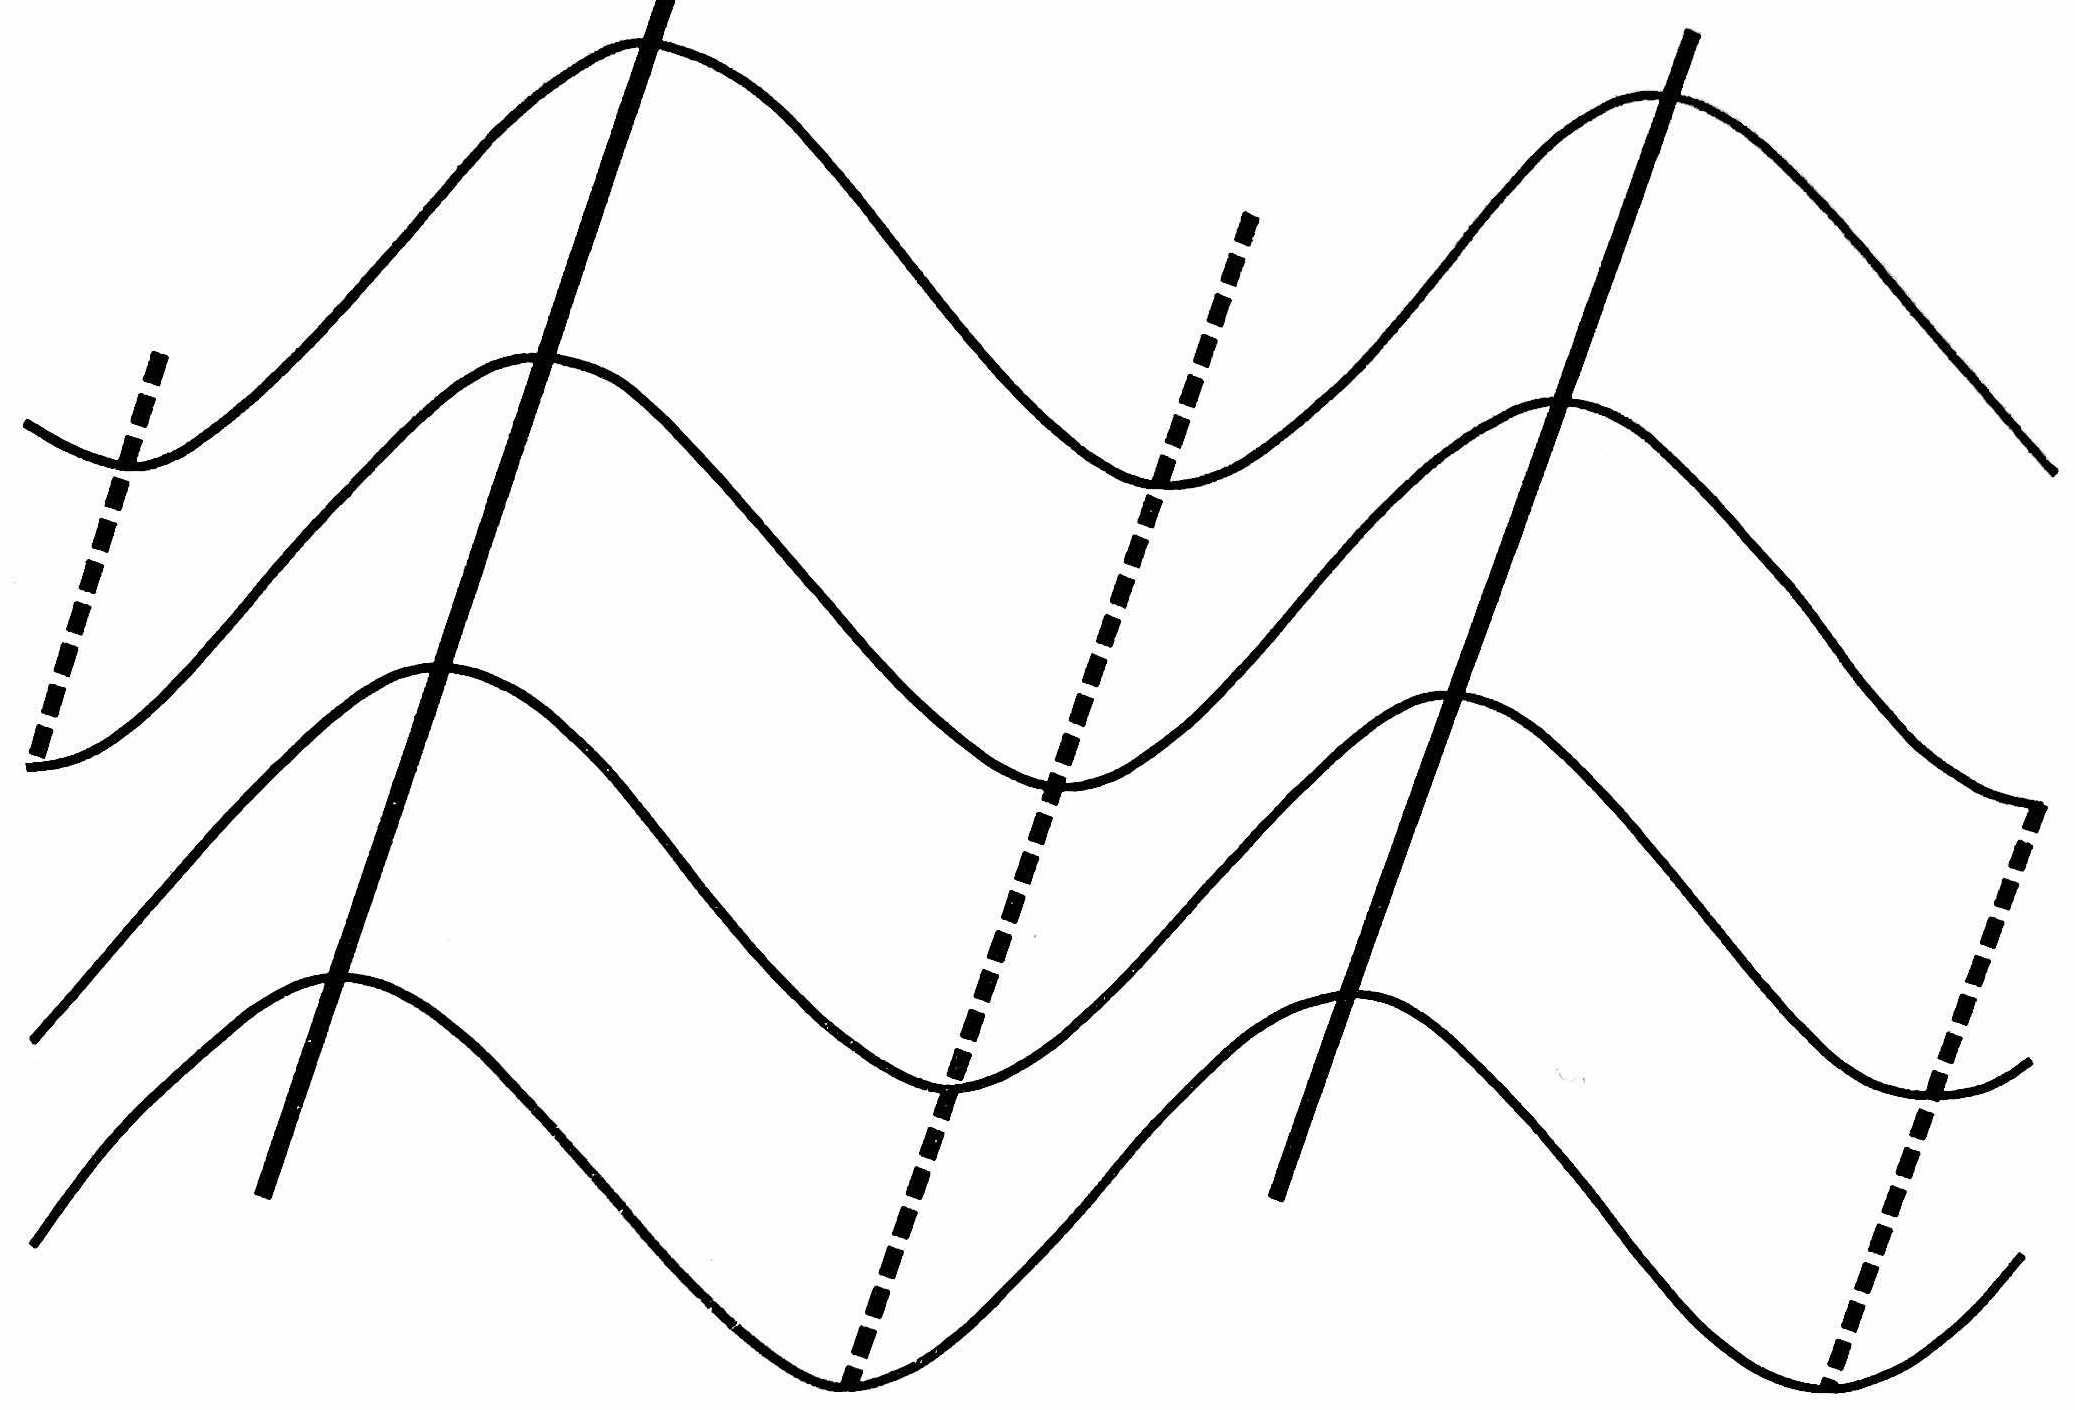
\includegraphics[width=0.7\textwidth]{images/ch04/p39_img01.jpeg}
  \caption{Schematic of NE--SW tilted trough and ridge axes in a midlatitude Rossby wave.  Solid lines indicate troughs (low geopotential) and dashed lines indicate ridges.  The systematic tilt yields a nonzero zonal-mean eddy momentum flux $(u_Ev_E)_Z > 0$, resulting in poleward (northward in NH) momentum transport. \hisu{중위도 로스비 파의 기압골/기압능 축 기울기 모식도.  NE--SW 방향으로 기울어진 기압골 축 (실선)은 $[u_Ev_E] > 0$을 만들어 극 방향 운동량 수송을 일으킨다.}}
  \label{fig:ch04_trough_tilt}
\end{figure}


% =============================================================================
%   SECTION 3 — Potential Vorticity Transport
% =============================================================================

\subsection{Potential Vorticity Transport}

The upgradient nature of momentum transport poses a major challenge for
parameterization.  The resolution comes from considering the transport of
\textgr{quasi-geostrophic potential vorticity (QGPV)}, which is
\textit{downgradient}---and whose transport encapsulates both heat and
momentum fluxes simultaneously.

% --------------------------------------------------------------------------
\subsubsection{Quasi-Geostrophic Potential Vorticity}

\begin{definition}[QG Potential Vorticity]
The quasi-geostrophic potential vorticity is defined as
\begin{equation}\label{eq:QGPV}
  Q = (\zeta_g + f) + \frac{\partial}{\partial p}
    \left(\frac{f^2}{\sigma}\frac{\partial\Psi}{\partial p}\right),
\end{equation}
where $\zeta_g$ is the geostrophic relative vorticity,
$\Psi = \Phi/f_0$ is the geostrophic streamfunction, and
$\sigma = -(\alpha/\theta)(\partial\theta/\partial p)$ is the static
stability parameter.
\end{definition}

\hisu{QG PV = 절대 소용돌이도 + 정적 안정도 항.  이것은 \textbf{합}으로 정의된다.
Ertel PV는 \textbf{곱}으로 정의되는 것과 대조적: $P_E = -g\eta_a\cdot\nabla\theta$.
QG PV는 Ertel PV의 선형화(quasi-geostrophic 근사)에 해당한다.}

% --------------------------------------------------------------------------
\subsubsection{Meridional PV Flux Decomposition}

The zonally averaged meridional PV flux can be decomposed into three
contributions:

\begin{equation}\label{eq:vQ_decomp}
  (vQ)_Z = \underbrace{f\,v_Z}_{\text{planetary}}
    + \underbrace{(v\zeta)_Z}_{\text{vorticity flux}}
    + \underbrace{\left[v\frac{\partial}{\partial p}
      \left(\frac{f^2}{\sigma}\frac{\partial\Psi}{\partial p}
      \right)\right]_Z}_{\text{thickness flux}}.
\end{equation}

We now show that each dynamical term reduces to a divergence of a
familiar flux.

\paragraph{First term: planetary vorticity.}
Since $f$ depends only on latitude, $fv_Z$ is simply the Coriolis
acceleration of the mean meridional flow.  In the vertically averaged,
steady-state budget this term is negligible ($v_Z \approx 0$).

\paragraph{Second term: vorticity flux $=$ convergence of momentum flux.}

\begin{proposition}[Vorticity Flux Identity]
\begin{equation}\label{eq:vort_flux}
  (v\zeta)_Z
  = -\frac{1}{a\cos^2\phi}\frac{\partial}{\partial\phi}
    \bigl((uv\cos^2\phi)_Z\bigr).
\end{equation}
\end{proposition}

\begin{proof}
In the QG framework on the beta plane, $\zeta_g = -\partial u/\partial y
+ \partial v/\partial x$ (approximating $y = a\phi$, $x = a\cos\phi\;\lambda$).
Then
\begin{align*}
  (v\zeta)_Z
  &= \left(v\frac{\partial v}{\partial x}\right)_Z
    - \left(v\frac{\partial u}{\partial y}\right)_Z \\
  &= \frac{\partial}{\partial x}\left(\frac{v^2}{2}\right)_Z
    - \frac{\partial(uv)_Z}{\partial y}
    + \left(u\frac{\partial v}{\partial y}\right)_Z.
\end{align*}
The first term vanishes under zonal averaging.
Using the nondivergent geostrophic wind ($\partial u/\partial x + \partial v/\partial y = 0$ in the QG limit),
the last term becomes $-\left(u\,\partial u/\partial x\right)_Z = -\partial(u^2/2)_Z/\partial x = 0$.
Hence, in spherical coordinates with the metric factor:
\[
  (v\zeta)_Z = -\frac{1}{a\cos^2\phi}\frac{\partial}{\partial\phi}
    \bigl((uv)_Z\cos^2\phi\bigr).\qedhere
\]
\end{proof}

\hisu{$(v\zeta)_Z$는 운동량 플럭스 $(uv)_Z$의 수렴과 같다!
즉, 소용돌이도 수송을 알면 운동량 수송을 안다.}

\paragraph{Third term: thickness flux $=$ vertical derivative of heat flux.}

\begin{proposition}[Thickness Flux Identity]
\begin{equation}\label{eq:thick_flux}
  \left[v\frac{\partial}{\partial p}
    \left(\frac{f^2}{\sigma}\frac{\partial\Psi}{\partial p}\right)\right]_Z
  = -\frac{\partial}{\partial p}
    \left[\frac{Rf}{\sigma\,p}(vT)_Z\right].
\end{equation}
\end{proposition}

\begin{proof}
Using the hydrostatic relation $\partial\Psi/\partial p = \partial(\Phi/f_0)/\partial p = -\alpha/f_0 = -RT/(f_0 p)$
and integrating by parts in $\lambda$ (noting boundary terms vanish by
periodicity), one obtains
\[
  \left[v\frac{\partial}{\partial p}
    \left(\frac{f^2}{\sigma}\frac{\partial\Psi}{\partial p}\right)\right]_Z
  = -\frac{\partial}{\partial p}
    \left(\frac{f^2}{\sigma}\frac{(v\,\partial\Psi/\partial p)_Z}{1}\right)
  = -\frac{\partial}{\partial p}
    \left[\frac{Rf}{\sigma\,p}(vT)_Z\right].\qedhere
\]
\end{proof}

\hisu{thickness flux는 열 플럭스 $(vT)_Z$의 연직 미분과 관련된다.
PV 수송 = 운동량 플럭스 수렴 + 열 플럭스의 연직 미분.  한 공식으로 둘 다 포함!}

% --------------------------------------------------------------------------
\subsubsection{Full PV Transport Formula}

Combining \eqref{eq:vort_flux} and \eqref{eq:thick_flux} (and neglecting
the planetary term for the eddy part):

\begin{equation}\label{eq:vQ_full}
  \boxed{
  (v_E Q_E)_Z
  = -\frac{1}{a\cos^2\phi}\frac{\partial}{\partial\phi}
    \bigl((u_E v_E)_Z\cos^2\phi\bigr)
  - \frac{\partial}{\partial p}
    \left[\frac{Rf}{\sigma\,p}(v_E T_E)_Z\right].
  }
\end{equation}

\begin{remark}
This is a key result: the eddy PV flux is \textit{entirely determined}
by the eddy momentum flux and eddy heat flux.
\end{remark}

% --------------------------------------------------------------------------
\subsubsection{Downgradient PV Transport and Parameterization}

Observations and theory show that \textgr{eddy PV transport is downgradient}:

\begin{equation}\label{eq:PV_param}
  (v_E Q_E)_Z \approx -K_Q\,\frac{1}{a}\frac{\partial Q_Z}{\partial\phi},
  \qquad K_Q > 0.
\end{equation}

\begin{theorem}[Resolution of the Upgradient Momentum Puzzle]
The meridional gradient of mean QG PV is dominated by the planetary
vorticity gradient $\beta = \partial f/\partial y$:
\[
  \frac{1}{a}\frac{\partial Q_Z}{\partial\phi}
  \approx \beta + \text{(smaller terms)}.
\]
Since the total PV flux is downgradient and includes both the
(downgradient) heat flux and the (upgradient) momentum flux, the
upgradient momentum transport is a \textbf{necessary consequence} of
downgradient PV transport combined with the dominance of $\beta$ in
the PV gradient.
\end{theorem}

\begin{hisublock}
왜 운동량이 upgradient로 수송되는지 이해하기:
\begin{enumerate}
  \item PV 수송은 downgradient (관측 사실 \& 이론).
  \item PV gradient $\approx \beta > 0$ (행성 소용돌이도 기울기가 지배적).
  \item 따라서 $(v_E Q_E)_Z < 0$ (남쪽으로, downgradient).
  \item PV 수송 = 운동량 수렴 + 열 수송의 연직 미분.
  \item 열 수송이 downgradient (양수)이므로, 운동량 수렴 항이 이를 보상해야 함.
  \item 결론: 운동량은 upgradient! 에디가 PV를 확산시키면서 동시에 운동량을 모은다.
\end{enumerate}
이것이 대기 대순환에서 제트 기류가 유지되는 근본 메커니즘이다!
\end{hisublock}


% =============================================================================
%   SECTION 4 — Eliassen-Palm (EP) Flux
% =============================================================================

\subsection{Eliassen--Palm (EP) Flux}

The EP flux framework provides the most elegant and complete description of
eddy--mean flow interaction in the zonally averaged circulation.

% --------------------------------------------------------------------------
\subsubsection{Zonally Averaged Equation Set}

The complete set of zonally averaged quasi-geostrophic equations on the
$\beta$-plane is:

\begin{align}
  \frac{\partial u_Z}{\partial t} - fv_Z
    &= \frac{1}{a\cos\phi}\frac{\partial}{\partial\phi}
       \bigl((u_E v_E)_Z\cos\phi\bigr)\cdot\frac{-\cos\phi}{\cos\phi}
       + F_{\lambda Z}
  \label{eq:EP_umom}\\[4pt]
  \frac{\partial\theta_Z}{\partial t}
    + \omega_Z\frac{\partial\bar{\theta}}{\partial p}
    &= -\frac{1}{a\cos\phi}\frac{\partial}{\partial\phi}
       \bigl((v_E\theta_E)_Z\cos\phi\bigr)
       + \frac{1}{c_p}H_Z
  \label{eq:EP_thermo}\\[4pt]
  \frac{1}{a\cos\phi}\frac{\partial}{\partial\phi}(v_Z\cos\phi)
    + \frac{\partial\omega_Z}{\partial p} &= 0
  \label{eq:EP_cont}\\[4pt]
  f\frac{\partial u_Z}{\partial p}
    &= \frac{R}{p}\frac{1}{a}\frac{\partial T_Z}{\partial\phi}
  \label{eq:EP_twind}
\end{align}

\hisu{%
\eqref{eq:EP_umom}: 동서 운동량 방정식 (에디 운동량 플럭스 강제 포함)\\
\eqref{eq:EP_thermo}: 열역학 방정식 (에디 열 플럭스 강제 포함)\\
\eqref{eq:EP_cont}: 연속 방정식 (평균 자오면 순환 $v_Z, \omega_Z$ 결정)\\
\eqref{eq:EP_twind}: 온도풍 관계 (진단 관계식)
}

Rearranging \eqref{eq:EP_umom} more explicitly:
\begin{equation}\label{eq:umom_explicit}
  \frac{\partial u_Z}{\partial t}
  = fv_Z
    - \frac{1}{a\cos^2\phi}\frac{\partial}{\partial\phi}
      \bigl((u_E v_E)_Z\cos^2\phi\bigr)
    + F_{\lambda Z}.
\end{equation}

% --------------------------------------------------------------------------
\subsubsection{The Non-Acceleration Theorem}

\begin{theorem}[Non-Acceleration Theorem (Charney and Drazin, 1961)]
Under steady, conservative (adiabatic, non-dissipative) conditions
($H = 0$, $F_\lambda = 0$, $\partial/\partial t = 0$):
\begin{enumerate}
  \item The eddy fluxes force a mean meridional circulation
    ($v_Z$, $\omega_Z$), but
  \item they do \textbf{not} force the zonal-mean zonal wind $u_Z$ or the
    zonal-mean temperature $\theta_Z$.
\end{enumerate}
That is, the momentum flux convergence is \textbf{exactly counterbalanced}
by the Coriolis torque of the induced mean meridional circulation:
\begin{equation}\label{eq:non_accel}
  fv_Z = \frac{1}{a\cos^2\phi}\frac{\partial}{\partial\phi}
    \bigl((u_E v_E)_Z\cos^2\phi\bigr)
  \qquad\Longrightarrow\qquad
  \frac{\partial u_Z}{\partial t} = 0.
\end{equation}
\end{theorem}

\begin{hisublock}
비가속 정리의 의미:
\begin{itemize}
  \item 단열, 비마찰 조건에서 에디는 평균류를 가속시키지 못한다!
  \item 에디가 운동량을 수렴시키면, 그에 의해 유도된 평균 자오면 순환의
    코리올리 힘이 정확히 상쇄한다.
  \item 따라서 평균류가 변하려면 반드시 마찰이나 비단열 가열이 있어야 한다.
  \item 이것은 대기 역학에서 가장 중요한 정리 중 하나!
\end{itemize}
\end{hisublock}

\begin{proof}[Sketch]
From \eqref{eq:EP_umom} with $F_{\lambda Z} = 0$ and
$\partial u_Z/\partial t = 0$:
\[
  fv_Z = \frac{1}{a\cos^2\phi}\frac{\partial}{\partial\phi}
    \bigl((u_E v_E)_Z\cos^2\phi\bigr).
\]
From \eqref{eq:EP_thermo} with $H_Z = 0$ and
$\partial\theta_Z/\partial t = 0$:
\[
  \omega_Z\frac{\partial\bar{\theta}}{\partial p}
  = -\frac{1}{a\cos\phi}\frac{\partial}{\partial\phi}
    \bigl((v_E\theta_E)_Z\cos\phi\bigr).
\]
These determine $v_Z$ and $\omega_Z$ in terms of the eddy fluxes, but
$u_Z$ and $\theta_Z$ remain unchanged.  The eddies drive a mean
meridional circulation that exactly compensates their direct forcing
of the mean state.
\end{proof}

% --------------------------------------------------------------------------
\subsubsection{Definition of the EP Flux Vector}

\begin{definition}[Eliassen--Palm Flux]
The \textgr{EP flux vector} $\mathbf{F}$ is defined (in the
$\phi$--$p$ plane) as
\begin{equation}\label{eq:EP_flux}
  \boxed{
  \mathbf{F} = \Bigl(\underbrace{-a(u_E v_E)_Z\cos\phi}_{F^{(\phi)}},\;
  \underbrace{\frac{fa\cos\phi\,(v_E\theta_E)_Z}
    {\partial\bar{\theta}/\partial p}}_{F^{(p)}}\Bigr).
  }
\end{equation}
The meridional component $F^{(\phi)}$ is related to the eddy momentum
flux, and the vertical component $F^{(p)}$ is related to the eddy
heat flux.
\end{definition}

\hisu{EP 플럭스 벡터의 두 성분:\\
$F^{(\phi)}$: $-(u_Ev_E)_Z$ 에 비례 $\to$ 운동량 플럭스\\
$F^{(p)}$: $(v_E\theta_E)_Z$ 에 비례 $\to$ 열 플럭스\\
이 두 에디 플럭스를 하나의 벡터로 통합한 것이 EP 플럭스!}

% --------------------------------------------------------------------------
\subsubsection{EP Flux Divergence and Wave Activity}

The zonally averaged zonal momentum equation can be written compactly as

\begin{equation}\label{eq:EP_div_momentum}
  \frac{\partial u_Z}{\partial t} - fv_Z
  = \frac{1}{a\cos\phi}\nabla\cdot\mathbf{F} + F_{\lambda Z},
\end{equation}

\noindent
where
\begin{equation}\label{eq:EP_divergence}
  \nabla\cdot\mathbf{F}
  \equiv \frac{1}{a\cos\phi}\frac{\partial}{\partial\phi}
    \bigl(F^{(\phi)}\cos\phi\bigr)
  + \frac{\partial F^{(p)}}{\partial p}.
\end{equation}

\begin{theorem}[Non-Acceleration in EP Flux Form]
The non-acceleration condition is equivalent to
\begin{equation}\label{eq:non_accel_EP}
  \nabla\cdot\mathbf{F} = 0.
\end{equation}
The zonal-mean flow is accelerated (decelerated) where the EP flux is
convergent (divergent):
\[
  \frac{\partial u_Z}{\partial t} \propto \nabla\cdot\mathbf{F}.
\]
\end{theorem}

\hisu{$\nabla\cdot\mathbf{F} > 0$: 서풍 가속 (EP flux가 발산하는 곳)\\
$\nabla\cdot\mathbf{F} < 0$: 동풍 가속 (EP flux가 수렴하는 곳, 파동이 소산/쇄파)\\
$\nabla\cdot\mathbf{F} = 0$: 비가속 조건 (보존적 파동의 전파)}

\begin{figure}[ht]
  \centering
  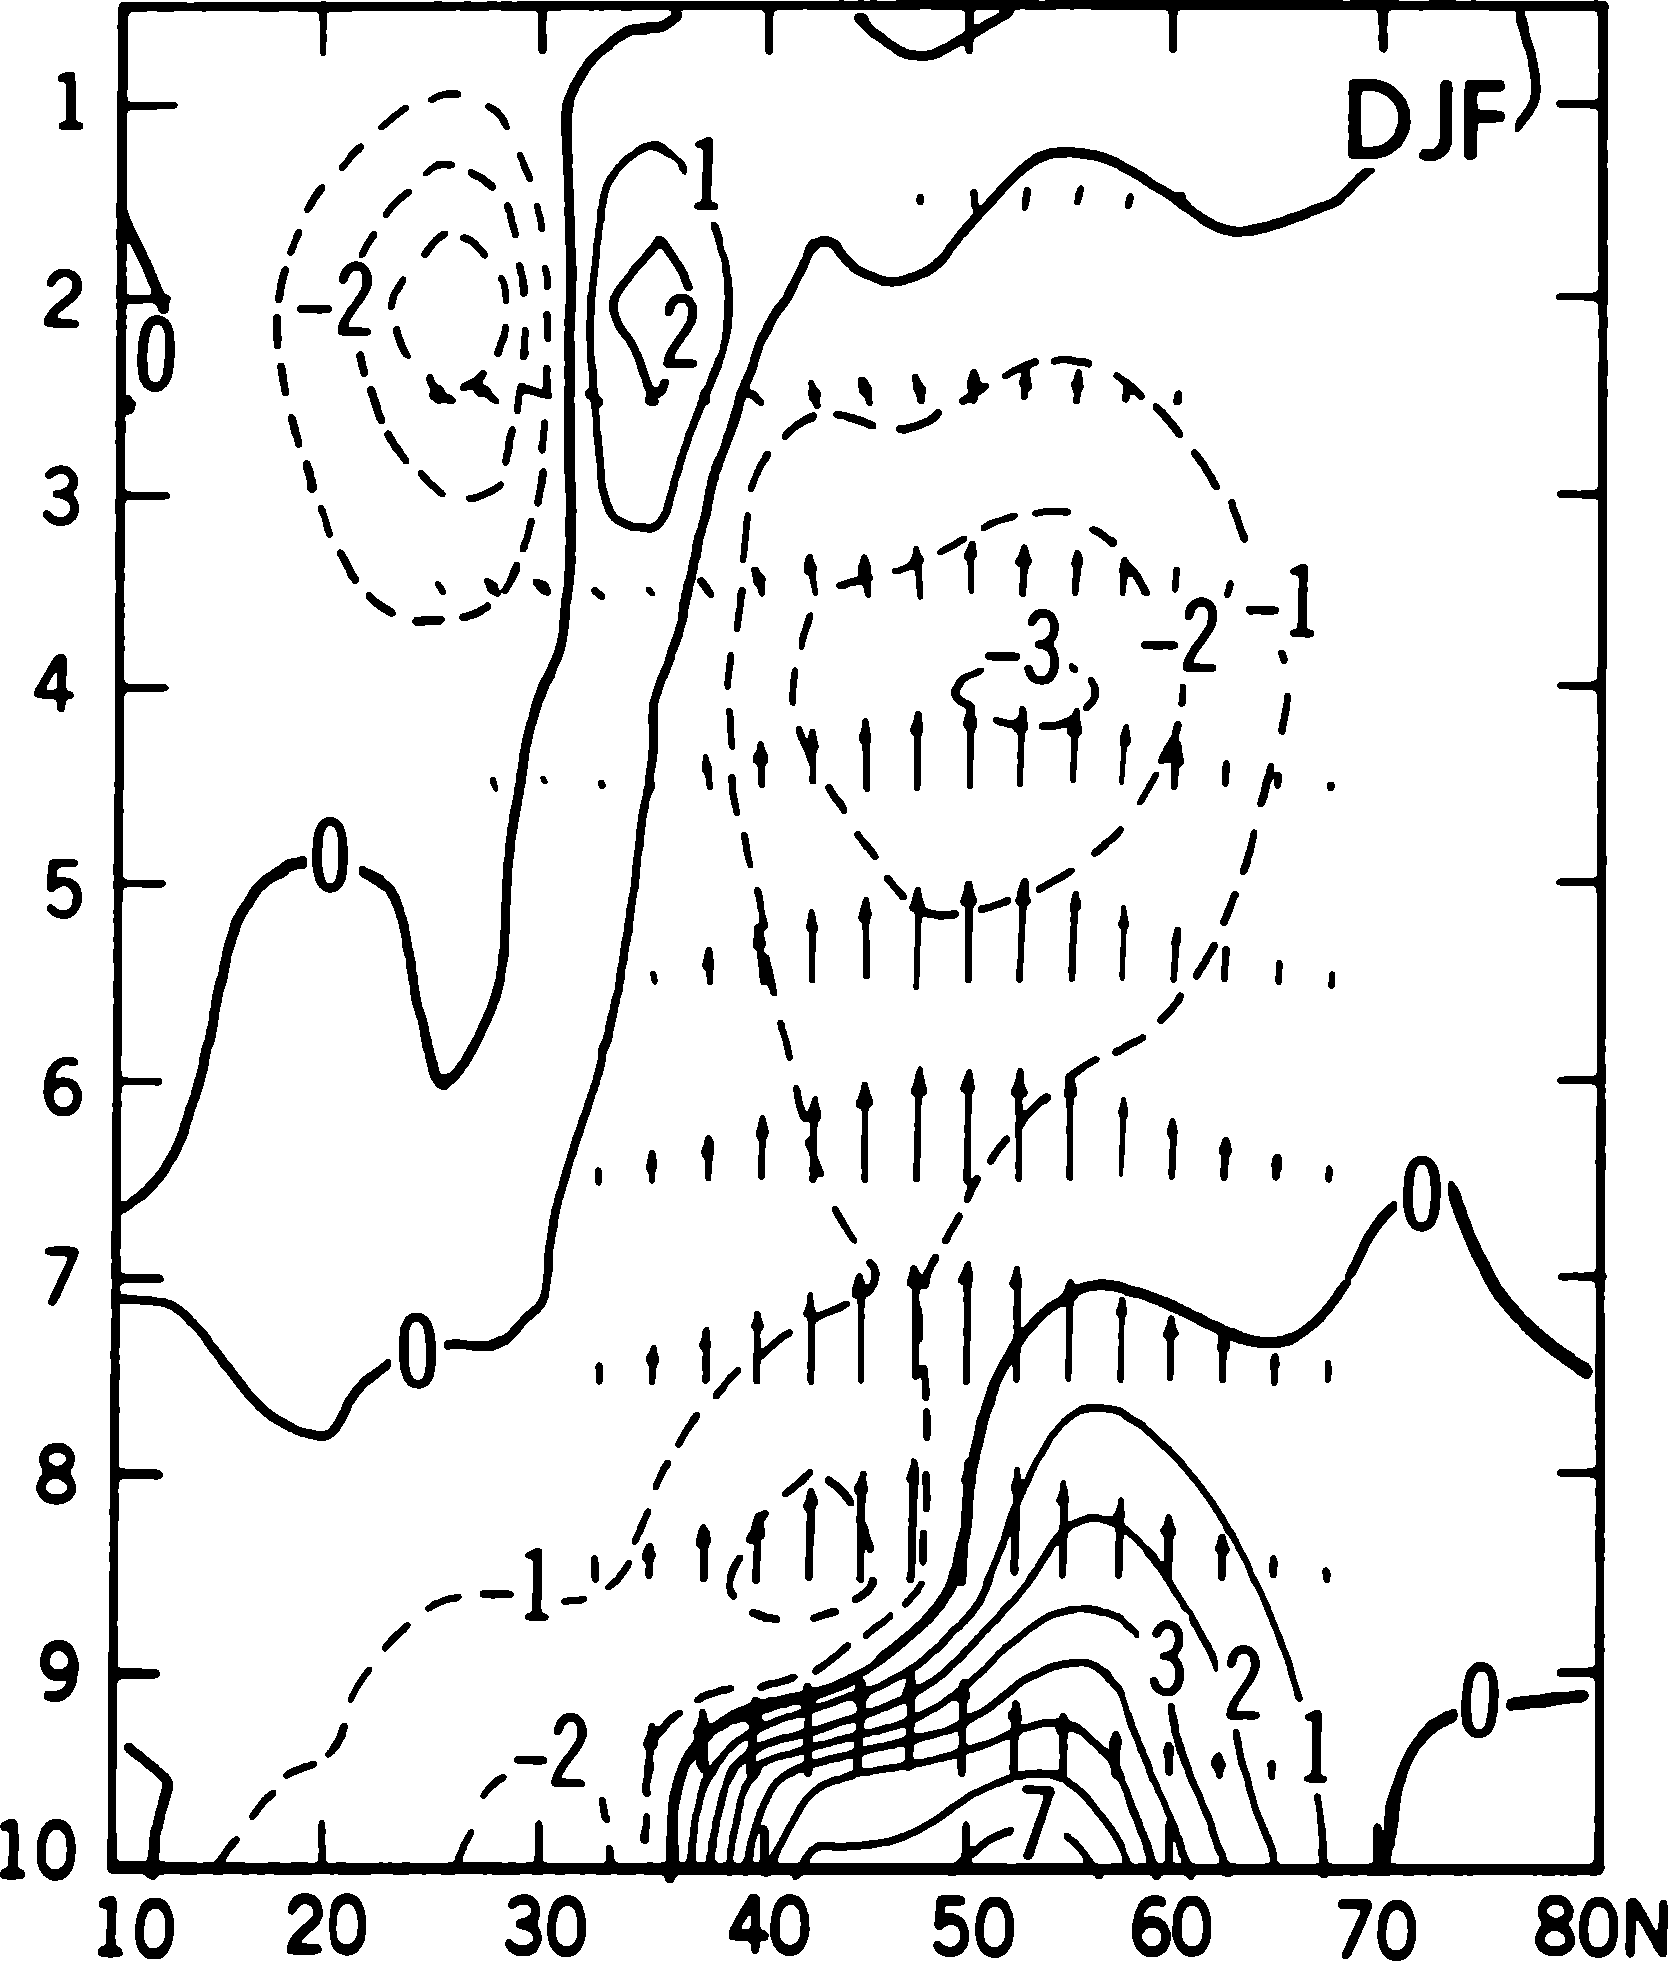
\includegraphics[width=0.48\textwidth]{images/ch04/p90_img01.png}\hfill
  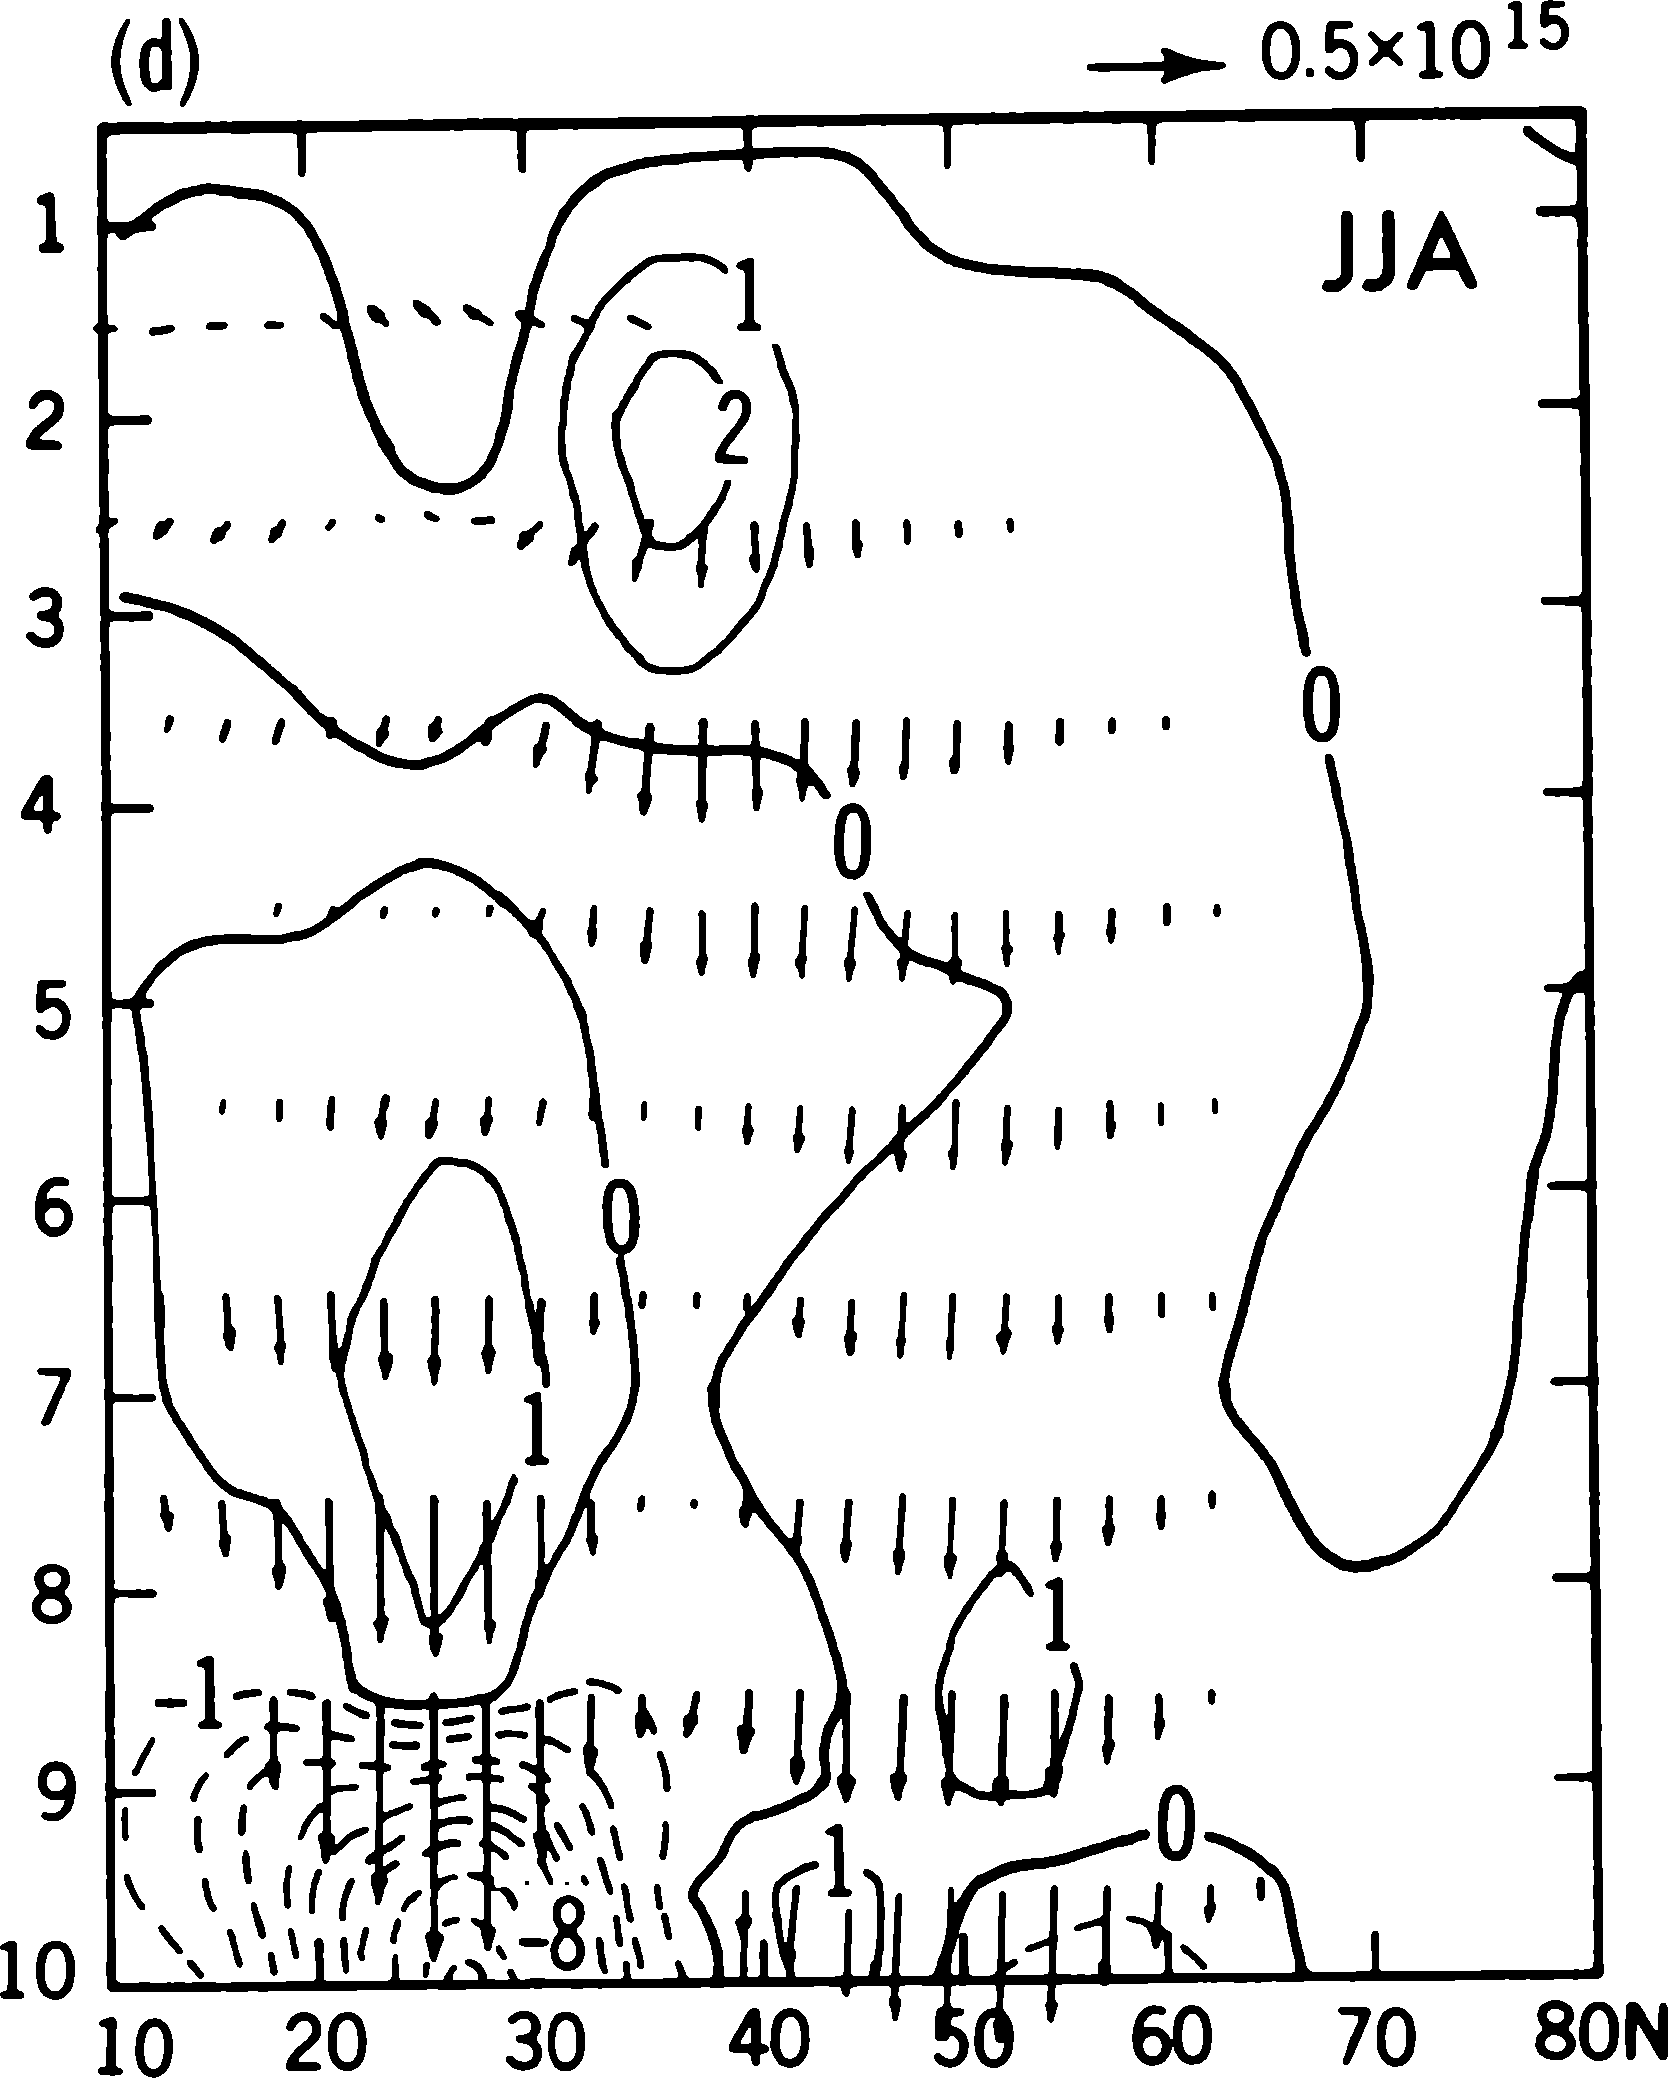
\includegraphics[width=0.48\textwidth]{images/ch04/p90_img02.png}
  \caption{EP flux cross-sections (arrows) and EP flux divergence (contours, m\,s$^{-1}$\,day$^{-1}$) for DJF (left) and JJA (right) in the Northern Hemisphere.  Arrows indicate wave-activity propagation: dominantly upward (poleward heat flux) and equatorward (poleward momentum flux).  Convergence ($\nabla\cdot\mathbf{F} < 0$, dashed contours) indicates wave dissipation and easterly acceleration of the mean flow; divergence ($\nabla\cdot\mathbf{F} > 0$, solid contours) indicates westerly acceleration. \hisu{EP 플럭스 단면도 (화살표)와 EP 플럭스 발산 (등치선): DJF (좌)와 JJA (우).  화살표는 파동 활동도의 전파 방향을 나타내며, 주로 위쪽 (열 플럭스)과 적도 쪽 (운동량 플럭스)을 향한다.  수렴 영역에서 동풍 가속, 발산 영역에서 서풍 가속이 발생한다.}}
  \label{fig:ch04_ep_flux_xsec}
\end{figure}

\begin{remark}[Interpretation of EP Flux Diagrams]
In EP flux cross-section diagrams:
\begin{itemize}
  \item Arrows show the direction of wave-activity propagation.
  \item \textgr{Upward} arrows indicate poleward heat flux
    ($(v_E\theta_E)_Z > 0$ in NH).
  \item \textgr{Equatorward} arrows indicate poleward momentum flux
    ($(u_E v_E)_Z > 0$ in NH $\Rightarrow$ $F^{(\phi)} < 0$).
  \item Divergence/convergence of arrows indicates wave sources/sinks,
    hence acceleration/deceleration of the mean flow.
\end{itemize}
\end{remark}

% --------------------------------------------------------------------------
\subsubsection{The General Case: Heating and Friction}

In the general (non-conservative) case, the mean meridional circulation
($v_Z$, $\omega_Z$) is forced by three agents:

\begin{enumerate}
  \item \textgr{Mean diabatic heating} $\overline{H}_{ZM}$
  \item \textgr{Mean friction} $F_{\lambda Z}$
  \item \textgr{Eddy forcing} via $\nabla\cdot\mathbf{F}$
\end{enumerate}

\noindent
The mean meridional circulation satisfies
\begin{align}
  fv_Z &= \frac{1}{a\cos\phi}\nabla\cdot\mathbf{F}
    + F_{\lambda Z} - \frac{\partial u_Z}{\partial t},
  \label{eq:gen_vmean}\\[4pt]
  \omega_Z\frac{\partial\bar{\theta}}{\partial p}
    &= \frac{1}{c_p}H_Z
    - \frac{1}{a\cos\phi}\frac{\partial}{\partial\phi}
      \bigl((v_E\theta_E)_Z\cos\phi\bigr)
    - \frac{\partial\theta_Z}{\partial t}.
  \label{eq:gen_omegamean}
\end{align}

\begin{remark}[The Ferrel Cell]
The midlatitude \textgr{Ferrel cell} is an indirect (thermally indirect)
circulation: warm air sinks and cold air rises.  It is \textbf{not}
driven by differential heating (like the Hadley cell) but is forced
primarily by the eddies through the EP flux divergence.
The eddy momentum flux convergence drives a poleward flow aloft
($fv_Z \approx \nabla\cdot\mathbf{F}/(a\cos\phi)$), which by
continuity requires descent in the subtropics and ascent at high
latitudes.
\end{remark}

\hisu{페렐 셀은 에디에 의해 구동되는 간접 순환!
열적으로는 따뜻한 곳에서 하강, 차가운 곳에서 상승하므로 `간접적'이다.
해들리 셀과 달리 직접적인 열적 구동이 아니라 에디 강제에 의한 응답이다.}


% =============================================================================
%   SECTION 5 — Transformed Eulerian Mean (TEM)
% =============================================================================

\subsection{Transformed Eulerian Mean (TEM) Formulation}

The standard Eulerian-mean equations mask the net effect of eddies
because the eddy-driven mean meridional circulation partially cancels
the direct eddy forcing (non-acceleration theorem).  The \textgr{TEM
formulation} introduces a \textbf{residual circulation} that reveals
the true eddy impact.

% --------------------------------------------------------------------------
\subsubsection{Residual Mean Meridional Circulation}

\begin{definition}[Residual Circulation]
The residual meridional and vertical velocities are defined as
\begin{align}
  v^* &\equiv v_Z - \frac{\partial}{\partial p}
    \left(\frac{(v_E\theta_E)_Z}{\partial\bar{\theta}/\partial p}\right),
  \label{eq:vstar}\\[4pt]
  \omega^* &\equiv \omega_Z + \frac{1}{a\cos\phi}
    \frac{\partial}{\partial\phi}
    \left(\frac{(v_E\theta_E)_Z\cos\phi}{\partial\bar{\theta}/\partial p}\right).
  \label{eq:omegastar}
\end{align}
\end{definition}

\hisu{잔차 순환 = Eulerian 평균 순환 $-$ 에디에 의한 Stokes drift 보정.
이것은 실제 물질 수송에 더 가까운 순환이다.}

\noindent
The TEM momentum and thermodynamic equations become:

\begin{align}
  \frac{\partial u_Z}{\partial t} - fv^*
    &= \frac{1}{a\cos\phi}\nabla\cdot\mathbf{F} + F_{\lambda Z},
  \label{eq:TEM_u}\\[4pt]
  \frac{\partial\theta_Z}{\partial t}
    + \omega^*\frac{\partial\bar{\theta}}{\partial p}
    &= \frac{1}{c_p}H_Z.
  \label{eq:TEM_theta}
\end{align}

\begin{remark}
In the TEM formulation, \eqref{eq:TEM_theta} contains \textbf{no
explicit eddy flux terms}---the eddy heat flux has been absorbed into
the definition of $\omega^*$.  The entire eddy effect on the mean flow
appears only through $\nabla\cdot\mathbf{F}$ in
\eqref{eq:TEM_u}.
\end{remark}

\begin{hisublock}
TEM의 장점:
\begin{itemize}
  \item 열역학 방정식에서 에디 항이 사라짐 $\to$ 잔차 순환이 단열 가열에 의해 직접 결정.
  \item 운동량 방정식에서 에디 효과가 오직 $\nabla\cdot\mathbf{F}$ 하나로 표현.
  \item 비가속 정리가 자명해짐: $\nabla\cdot\mathbf{F} = 0$이면 $v^* = 0$, $\omega^* = 0$,
    따라서 $\partial u_Z/\partial t = 0$.
  \item 잔차 순환은 Brewer--Dobson 순환과 밀접 (성층권에서 특히 유용).
\end{itemize}
\end{hisublock}


% =============================================================================
%   SECTION 6 — Globally Averaged Energy Balance
% =============================================================================

\subsection{Globally Averaged Energy Balance}

The maintenance of the general circulation ultimately rests on the
\textgr{differential radiative heating} between the tropics and poles.
This section provides a quantitative overview.

% --------------------------------------------------------------------------
\subsubsection{Top-of-Atmosphere Radiation Balance}

\begin{definition}[Net Radiation at TOA]
The net downward radiation at the top of the atmosphere is
\begin{equation}\label{eq:R_net}
  R_{\text{net}}(\phi) = S_{\text{abs}}(\phi) - F_{\text{OLR}}(\phi),
\end{equation}
where $S_{\text{abs}}$ is the absorbed shortwave (solar) radiation and
$F_{\text{OLR}}$ is the outgoing longwave radiation.
\end{definition}

The key observational facts:
\begin{itemize}
  \item \textbf{Absorbed solar radiation}: ranges from $> 300\;\text{W/m}^2$
    in the tropics to $< 100\;\text{W/m}^2$ at the poles---a factor of
    $\sim 3$ variation.
  \item \textbf{OLR}: much more uniform, ranging from $\sim 250\;\text{W/m}^2$
    in the tropics to $\sim 175\;\text{W/m}^2$ at the poles---less than
    a factor of 1.5 variation.
  \item \textbf{Net radiation crossover}: $R_{\text{net}} = 0$ at
    $\sim 38^\circ$ N/S latitude.  Equatorward: net surplus;
    poleward: net deficit.
\end{itemize}

\hisu{태양 복사는 적도--극 사이 3배 이상 차이가 나지만, OLR은 1.5배 차이에 불과.
이 불균형이 대기와 해양의 에너지 수송을 구동하는 원동력이다!}

\begin{figure}[ht]
  \centering
  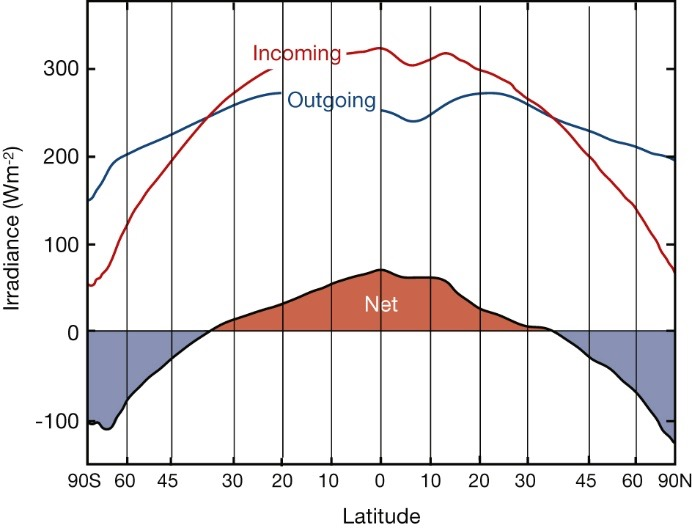
\includegraphics[width=0.85\textwidth]{images/ch04/p103_img01.jpeg}
  \caption{Zonally averaged TOA radiation balance as a function of latitude: absorbed solar (incoming, red), outgoing longwave radiation (blue), and net radiation (shaded).  The tropics have a net radiative surplus (red shading) and the extratropics a net deficit (blue shading), with the crossover near $\sim$38$^\circ$ latitude.  This differential heating is the fundamental driver of the general circulation. \hisu{위도별 TOA 복사 수지: 흡수 태양 복사 (적색), 사출 장파 복사 (청색), 순 복사 (음영).  열대의 복사 잉여와 고위도의 복사 적자가 $\sim$38$^\circ$에서 교차하며, 이 차등 가열이 대기 대순환의 근본 원동력이다.}}
  \label{fig:ch04_toa_radiation}
\end{figure}

% --------------------------------------------------------------------------
\subsubsection{Poleward Energy Transport}

From the requirement of global energy balance, the net poleward
energy transport across latitude $\phi$ is

\begin{equation}\label{eq:energy_transport}
  \mathcal{F}(\phi) = 2\pi a^2\int_{\phi}^{\pi/2}
    R_{\text{net}}(\phi')\cos\phi'\,d\phi'.
\end{equation}

\noindent
Observational estimates yield:
\begin{itemize}
  \item Total transport peaks at $\sim 5$--$6$ PW at $\sim 35^\circ$ latitude.
  \item \textgr{Atmospheric transport} dominates in the
    \textbf{extratropics} ($> 30^\circ$).
  \item \textgr{Oceanic transport} is significant mainly in the
    \textbf{tropics} ($< 20^\circ$), contributing $\sim 2$ PW.
\end{itemize}

\begin{hisublock}
에너지 수송의 분담:
\begin{itemize}
  \item 전구 총 수송 최대: $\sim$5--6 PW ($1\;\text{PW} = 10^{15}\;\text{W}$), $\sim 35^\circ$
  \item 대기: 중위도에서 지배적---주로 에디에 의한 현열 + 잠열 수송
  \item 해양: 열대에서 중요---서안 경계류 (걸프 스트림, 쿠로시오)
  \item 고위도에서는 거의 전부 대기가 담당
\end{itemize}
\end{hisublock}

\begin{figure}[ht]
  \centering
  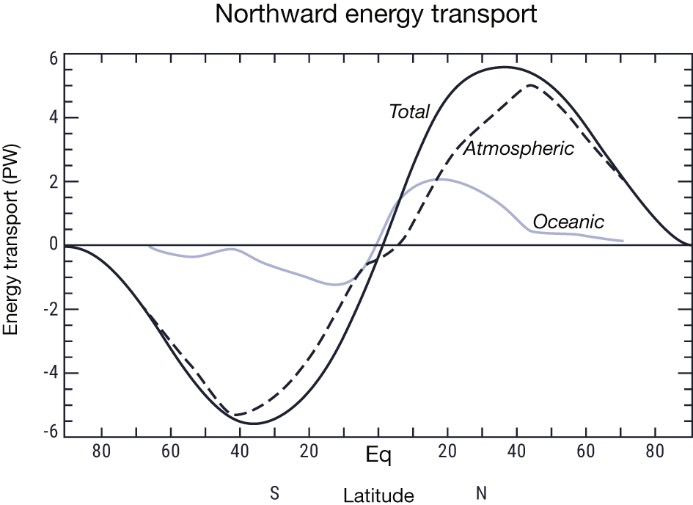
\includegraphics[width=0.85\textwidth]{images/ch04/p105_img01.jpeg}
  \caption{Observed northward energy transport (PW) as a function of latitude: total (dashed), atmospheric (solid black), and oceanic (grey).  The total poleward transport peaks at $\sim$5--6\,PW near 35$^\circ$ latitude; atmospheric transport dominates in the extratropics while oceanic transport contributes significantly in the tropics. \hisu{관측된 극 방향 에너지 수송 (PW): 총 수송 (점선), 대기 수송 (실선), 해양 수송 (회색).  총 수송은 $\sim$35$^\circ$에서 $\sim$5--6\,PW로 최대이며, 중위도에서는 대기, 열대에서는 해양이 지배적이다.}}
  \label{fig:ch04_energy_transport}
\end{figure}

\begin{figure}[ht]
  \centering
  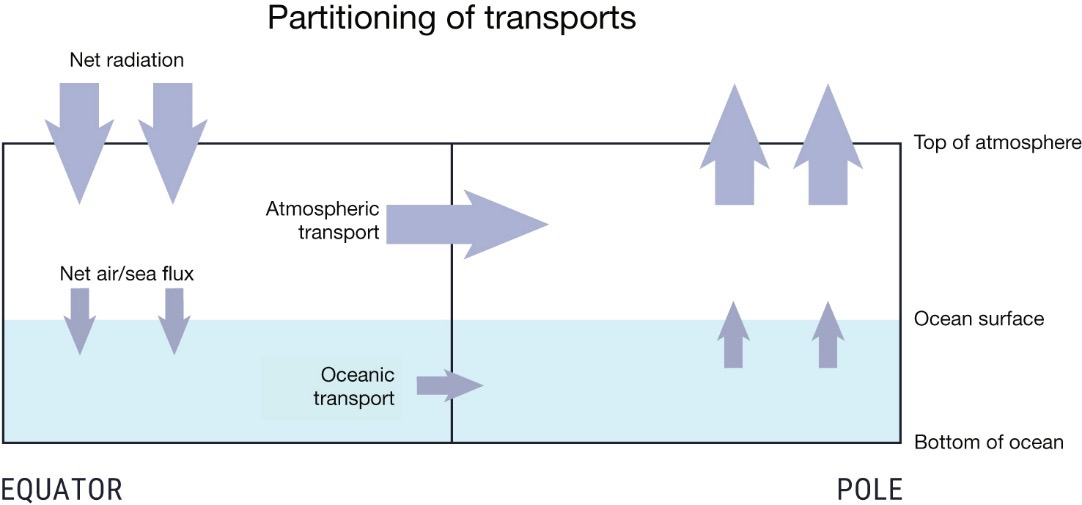
\includegraphics[width=0.85\textwidth]{images/ch04/p104_img01.jpeg}
  \caption{Schematic of the partitioning of poleward energy transports between the atmosphere and ocean.  Net radiation is absorbed at the top of the atmosphere (mostly in the tropics) and radiated back to space (mostly at higher latitudes).  The atmosphere and ocean each carry a portion of the required poleward transport, exchanging energy at the ocean surface through air--sea fluxes. \hisu{대기--해양 간 극 방향 에너지 수송 분배의 모식도.  적도에서 순 복사 에너지를 받아 대기 수송과 해양 수송으로 나뉘어 극 방향으로 운반된 후, 고위도에서 우주로 방출된다.}}
  \label{fig:ch04_transport_partition}
\end{figure}

% --------------------------------------------------------------------------
\subsubsection{Decomposition of Atmospheric Energy Transport}

The total atmospheric energy transport can be decomposed:

\begin{equation}\label{eq:atm_transport}
  \mathcal{F}_{\text{atm}} = \underbrace{\mathcal{F}_{\text{MMC}}}_{\text{mean meridional circ.}}
  + \underbrace{\mathcal{F}_{\text{SE}}}_{\text{stationary eddies}}
  + \underbrace{\mathcal{F}_{\text{TE}}}_{\text{transient eddies}}.
\end{equation}

\begin{multicols}{2}
\textgr{Tropics ($|\phi| < 30^\circ$):}
\begin{itemize}
  \item Hadley cell (MMC) dominates
  \item Transports dry static energy poleward
  \item Also large latent heat transport equatorward (lower branch)
\end{itemize}

\columnbreak

\textgr{Extratropics ($|\phi| > 30^\circ$):}
\begin{itemize}
  \item Transient eddies dominate
  \item Sensible heat $c_p(v_E T_E)_Z$
  \item Latent heat $L_v(v_E q_E)_Z$
  \item Potential energy $(v_E\Phi_E)_Z$
\end{itemize}
\end{multicols}

\hisu{열대에서는 해들리 셀, 중위도에서는 에디(특히 이동성 저기압)가 에너지 수송의 주역.}

% --------------------------------------------------------------------------
\subsubsection{Summary: The General Circulation as an Energy Engine}

\begin{remarkbox}
The atmosphere acts as a heat engine that:
\begin{enumerate}
  \item Absorbs energy preferentially in the tropics,
  \item Transports it poleward via mean circulations and eddies,
  \item Radiates it to space more uniformly across all latitudes.
\end{enumerate}
The eddies (baroclinic waves) are the primary agents of poleward
transport in the extratropics, maintaining the observed temperature
distribution against radiative forcing, and simultaneously maintaining
the jet streams through upgradient momentum transport.
\end{remarkbox}

\begin{hisublock}
\textbf{Chapter 4 핵심 정리}:
\begin{enumerate}
  \item 열 수송: downgradient, 에디가 지배, 확산으로 근사 가능.
  \item 운동량 수송: upgradient, 에디가 지배, 확산으로 근사 불가.
  \item PV 수송: downgradient, 운동량 + 열 수송을 통합.  PV 확산으로 upgradient 운동량 수송 설명 가능.
  \item EP 플럭스: 에디--평균류 상호작용의 통합적 기술.  $\nabla\cdot\mathbf{F}$가 평균류 가속을 결정.
  \item 비가속 정리: 보존적 파동은 평균류를 가속시키지 못함.  마찰/비단열이 있어야 변화.
  \item TEM: 잔차 순환이 실제 수송에 더 가까움.  에디 효과가 $\nabla\cdot\mathbf{F}$로 깔끔하게 표현.
  \item 에너지 균형: 적도--극 복사 불균형 $\to$ 대기/해양 수송 $\to$ 일반 순환 유지.
\end{enumerate}
\end{hisublock}

\vspace{6pt}
\noindent\textit{References:
Wallace, Battisti, Thompson, and Hartmann, ``The Atmospheric General
Circulation,'' Cambridge University Press;
Holton and Hakim, ``An Introduction to Dynamic Meteorology,''
Ch.~10.2--10.3;
Vallis, ``Atmospheric and Oceanic Fluid Dynamics,'' Ch.~12--13.}
